% Chapter 5

\chapter{Results} % Write in your own chapter title
\label{Chapter5}
\lhead{Chapter 5. \emph{Results}} % Write in your own chapter title to set the page header

In this chapter the results from the conducted experiments from Section~\ref{sec:experimentsetup} are presented.

\section{Cluster Quality - Real Dataset}
\label{sec:cq_realdataset}
Here are the result after incrementally cluster the ten multiple data batches of real game data and measuring the SSE error after performing $n$-iterations on each data batch. The SSE error gives an idea of the cluster quality at each data batch when using the k-means centroids results from previous data batch as an input.

Three different variations of $n$ were compared to see if there is any difference in doing a few iterations versus many iterations over each data batch. The main idea is to have a method that has a stable SSE error over multiple batches of data and have the desirable feature of having a downward trend for the SSE. 

Ten test runs were performed with different initial centroids from the first data batch trying to have the centroids to start at different points in space, creating different clusters and centroids as output from the first batch which can affect the consecutively batches. 

As we can see from Figure~\ref{fig:AvgSSEEachDataBatch} all the methods have a downward trend but are increasing the error with different amounts in batch $7-10$, tho the \textit{Iteration~1} method is showing a more stable change towards the final batch.


\begin{figure}[ht]
\centering
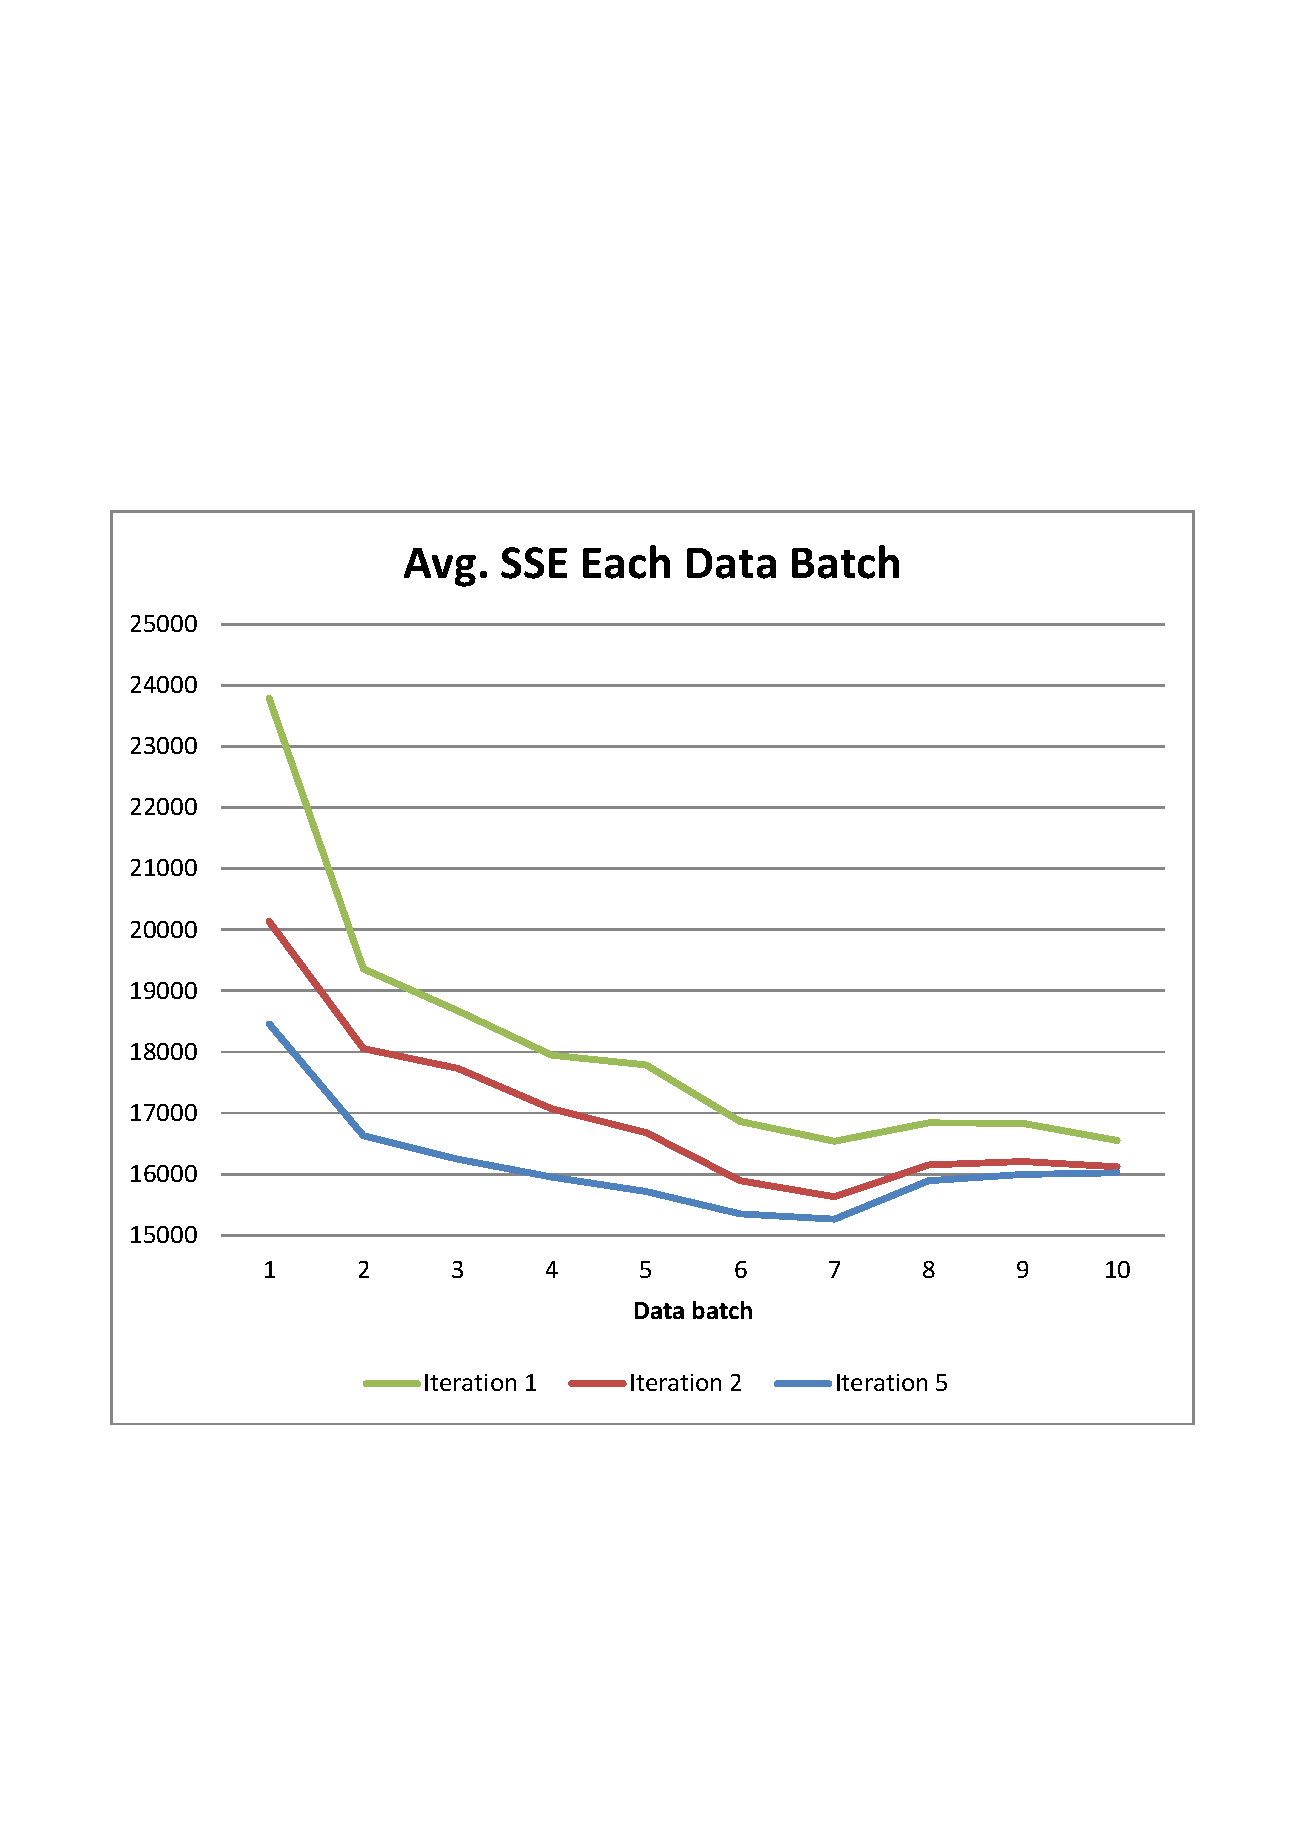
\includegraphics[trim = 10mm 70mm 10mm 80mm, clip, width=0.75\textwidth]{Figures/experiments/zdataWO_AvgSSEEachDataBatch.pdf}
\caption{This figure compares the average SSE error after clustering each data batch, using the three different $n$-iterations methods. }
\label{fig:AvgSSEEachDataBatch}
\end{figure}

After incrementally clustering the ten data batches with the different $n$-iterations methods, they all represent very similar clusters in the last batch, see Table~\ref{tab:results_avgSSEeachDataBatch}. The \textit{Iteration~2} and \textit{Iteration~5} has only about $0.6\%$ difference even tho the \textit{Iteration 5} is constantly showing lower SSE error in the first $7$ batches but then takes a steeper SSE increase up to the last batch. In this case the \textit{Iteration~5} method was too aggressive by trying to fit the centroids from the previous batch to the current batch by doing $5$-iterations.

\begin{table}[h]
\centering
\begin{tabular}{| l | r | r |}
    \hline
    & \textit{Iteration 2} & \textit{Iteration 5} \\ \hline
    \textit{Iteration 1} & $2.60\%$ & $3.19\%$  \\ \hline
    \textit{Iteration 2} & & $0.60\%$ \\ \hline
\end{tabular}
\caption{This table shows the average SSE error difference on the last data batch, between the three methods.}
\label{tab:results_avgSSEeachDataBatch}
\end{table}


In Figure~\ref{fig:results_AvgIncreaseEachTestRun} we can see on average how much was a single increase between one set of data batches for all test runs. The average single increase for the \textit{Iteration~1} method in each test is very different than the other methods. The reason is that are different initial centroids for each test and the \textit{Iteration~1} method only performs one iteration each time when clustering a data batch, doing so the method takes only one step towards the current data batch, slowly changing the means. If a data batch introduces a much different distribution this method will give worse results than the others because they are taking more steps towards the new data, but risking to deviate too much from the general population seen so far.


\begin{figure}[ht]
\centering
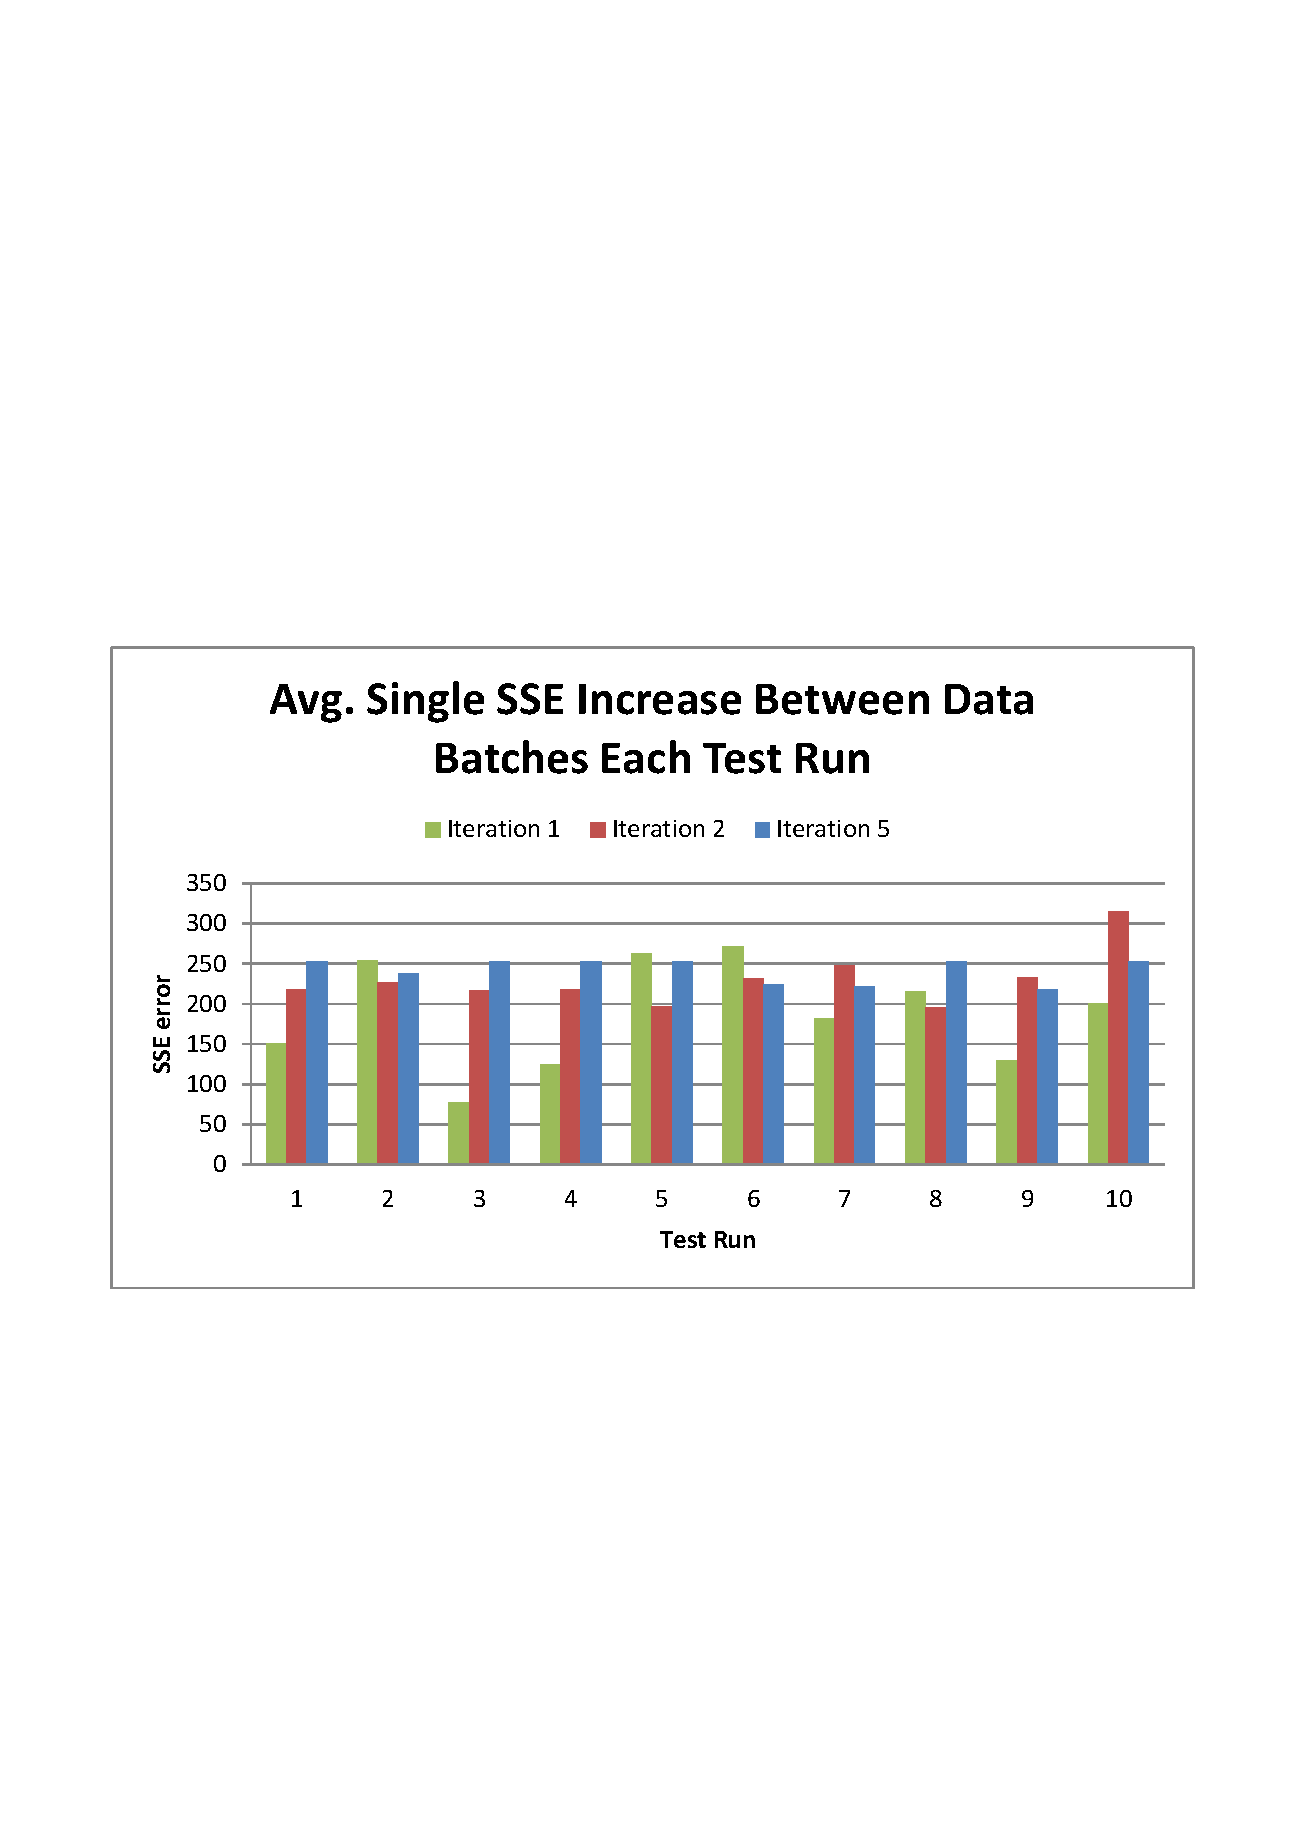
\includegraphics[trim = 10mm 90mm 10mm 100mm, clip, width=0.75\textwidth]{Figures/experiments/zdataWO_AvgSingleSSEIncreaseBetweenDataBatchesEachTestRun.pdf}
\caption{Here we can see on average the single SSE error increase that was measured, when SSE increases from one batch to another, for all the test runs.}
\label{fig:results_AvgIncreaseEachTestRun}
\end{figure}


When looking at the Figure~\ref{fig:results_AvgIncreaseBetweenDataBatches} we can see the single SSE error increase on average over all the ten test runs. The \textit{Iteration~1} method has considerable lower single SSE error increase compared to the \textit{Iteration~2} and\textit{Iteration~5} methods. The latter two methods being very similar to each other, both moving the centroids more aggressively away from already seen centroids.


\begin{figure}[ht]
\centering
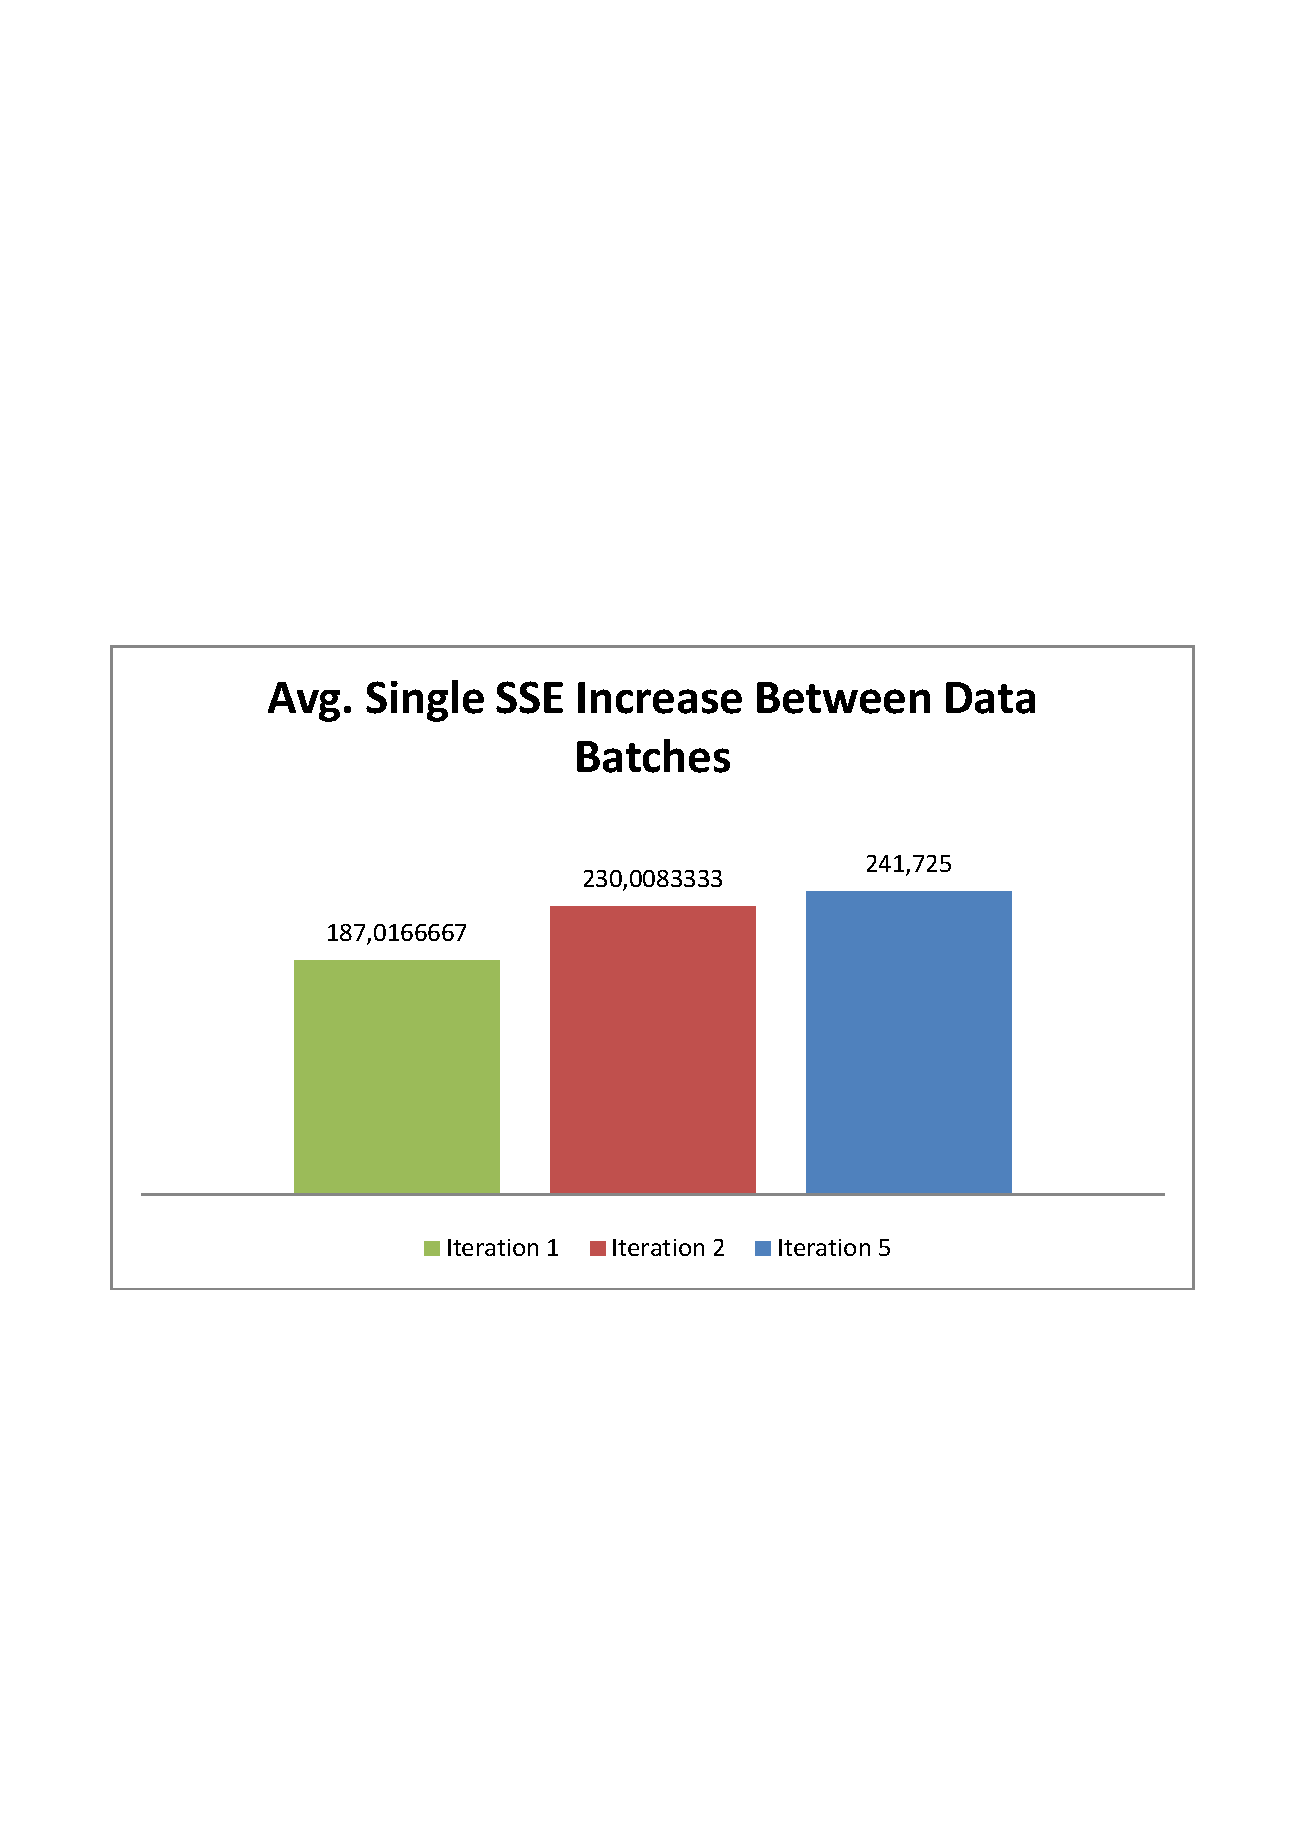
\includegraphics[trim = 10mm 90mm 10mm 100mm, clip, width=0.75\textwidth]{Figures/experiments/zdataWO_AvgSingleSSEIncreaseBetweenDataBatches.pdf}
\caption{Here we can see the average SSE error increase between two data batches, for the all the test runs. }
\label{fig:results_AvgIncreaseBetweenDataBatches}
\end{figure}

The results show that the \textit{Iteration 1} method has the lowest average single SSE error increase between a set of data batches. We now look at the aggregated SSE increase for each of the test runs, see ~Figure~\ref{fig:TotalSSEIncreaseEachTestRun}. 

\begin{figure}[ht]
\centering
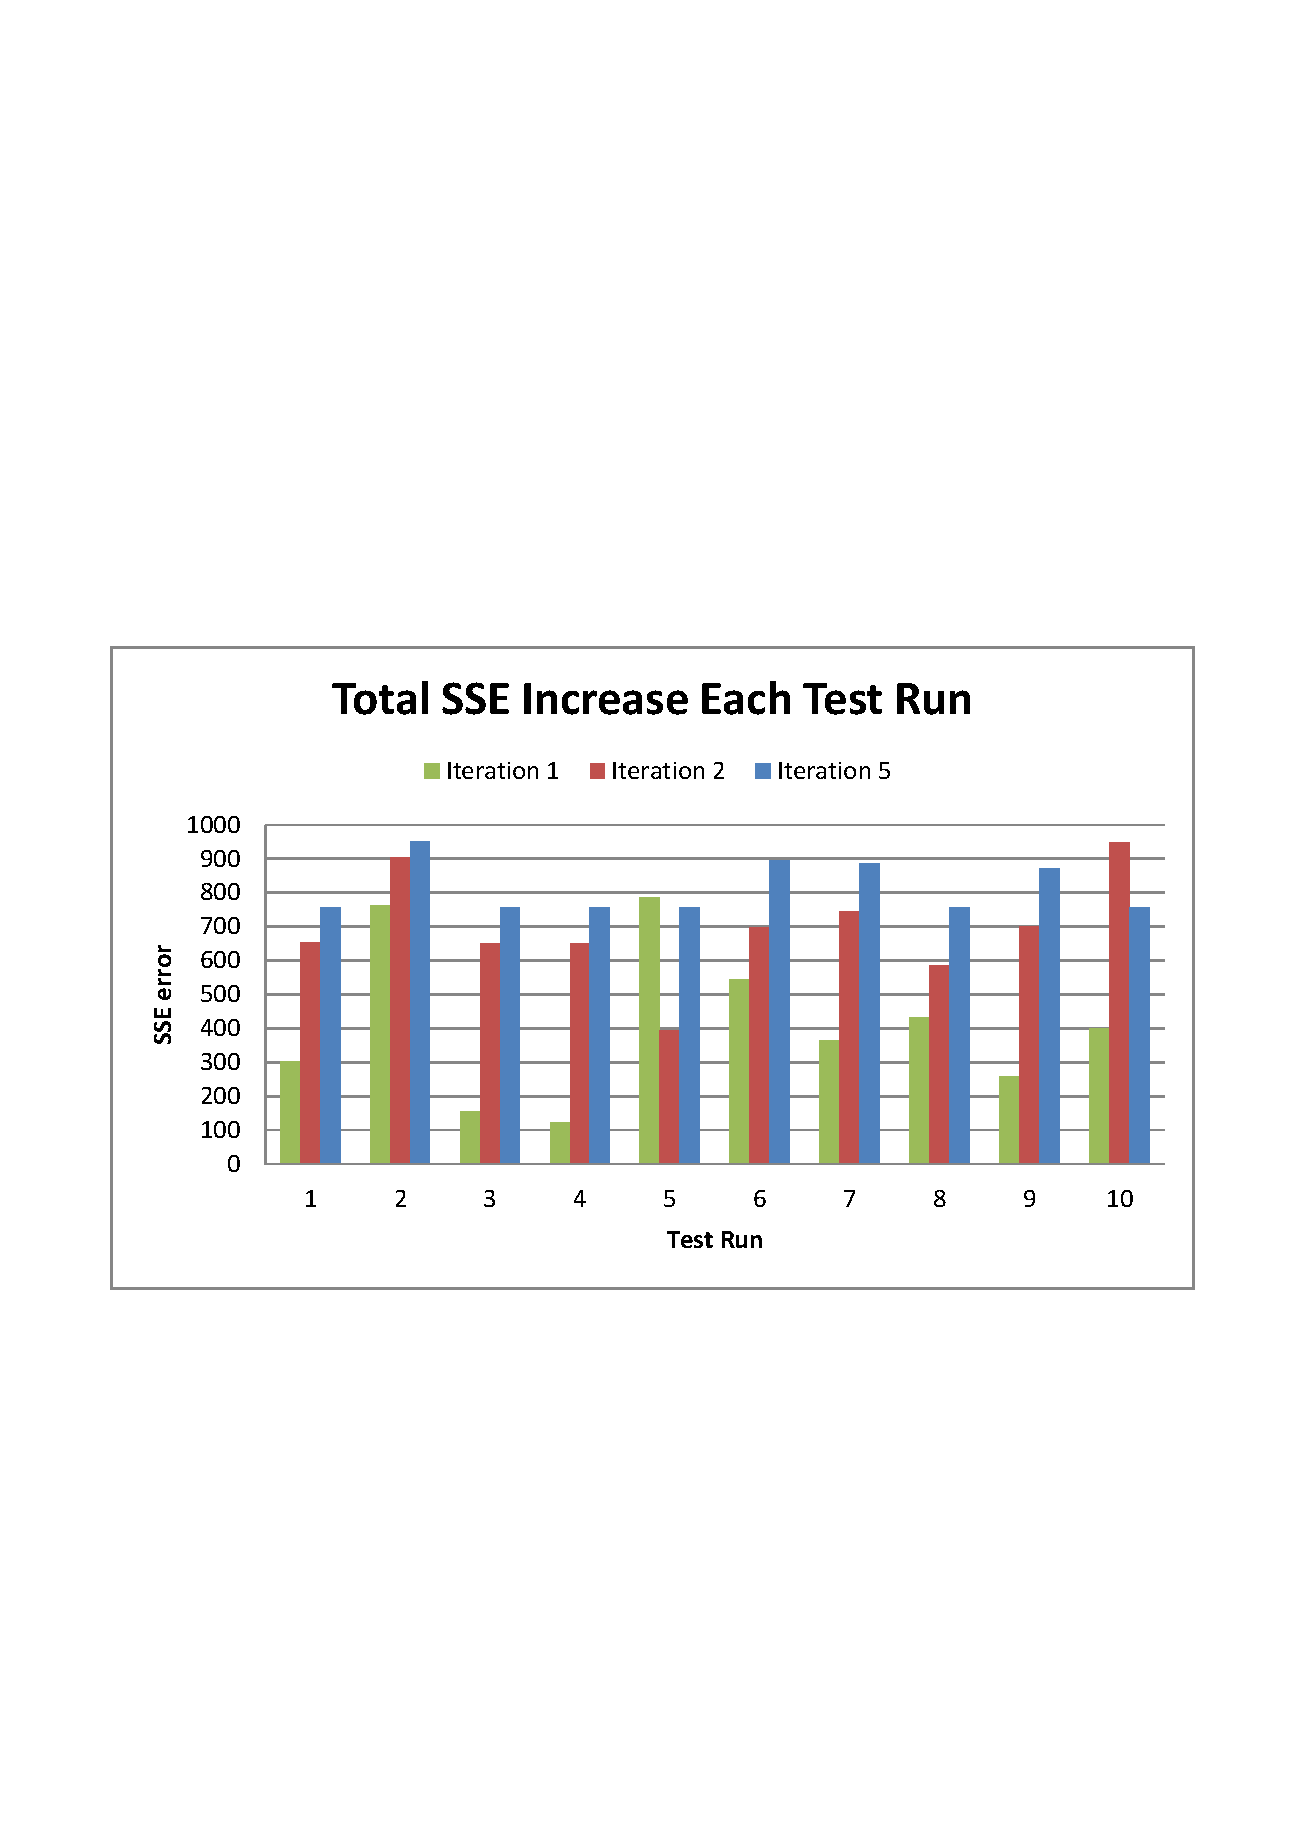
\includegraphics[trim = 10mm 90mm 10mm 100mm, clip, width=0.75\textwidth]{Figures/experiments/zdataWO_TotalSSEIncreaseEachTestRun.pdf}
\caption{This figure shows the aggregated SSE error between two data batches for each test run.}
\label{fig:TotalSSEIncreaseEachTestRun}
\end{figure}

The \textit{Iteration~1} method shows the lowest aggregated SSE error increase in all test runs, except in test run $5$. The random initial centroids from the first batch poorly represents the main distribution in the data and by performing $1$-iteration takes a longer time to adjust the centroids towards the mean of population. In Figure~\ref{fig:AvgSSEIncrease} is the average aggregate SSE error shown, over all the ten runs peformed.


\begin{figure}[ht]
\centering
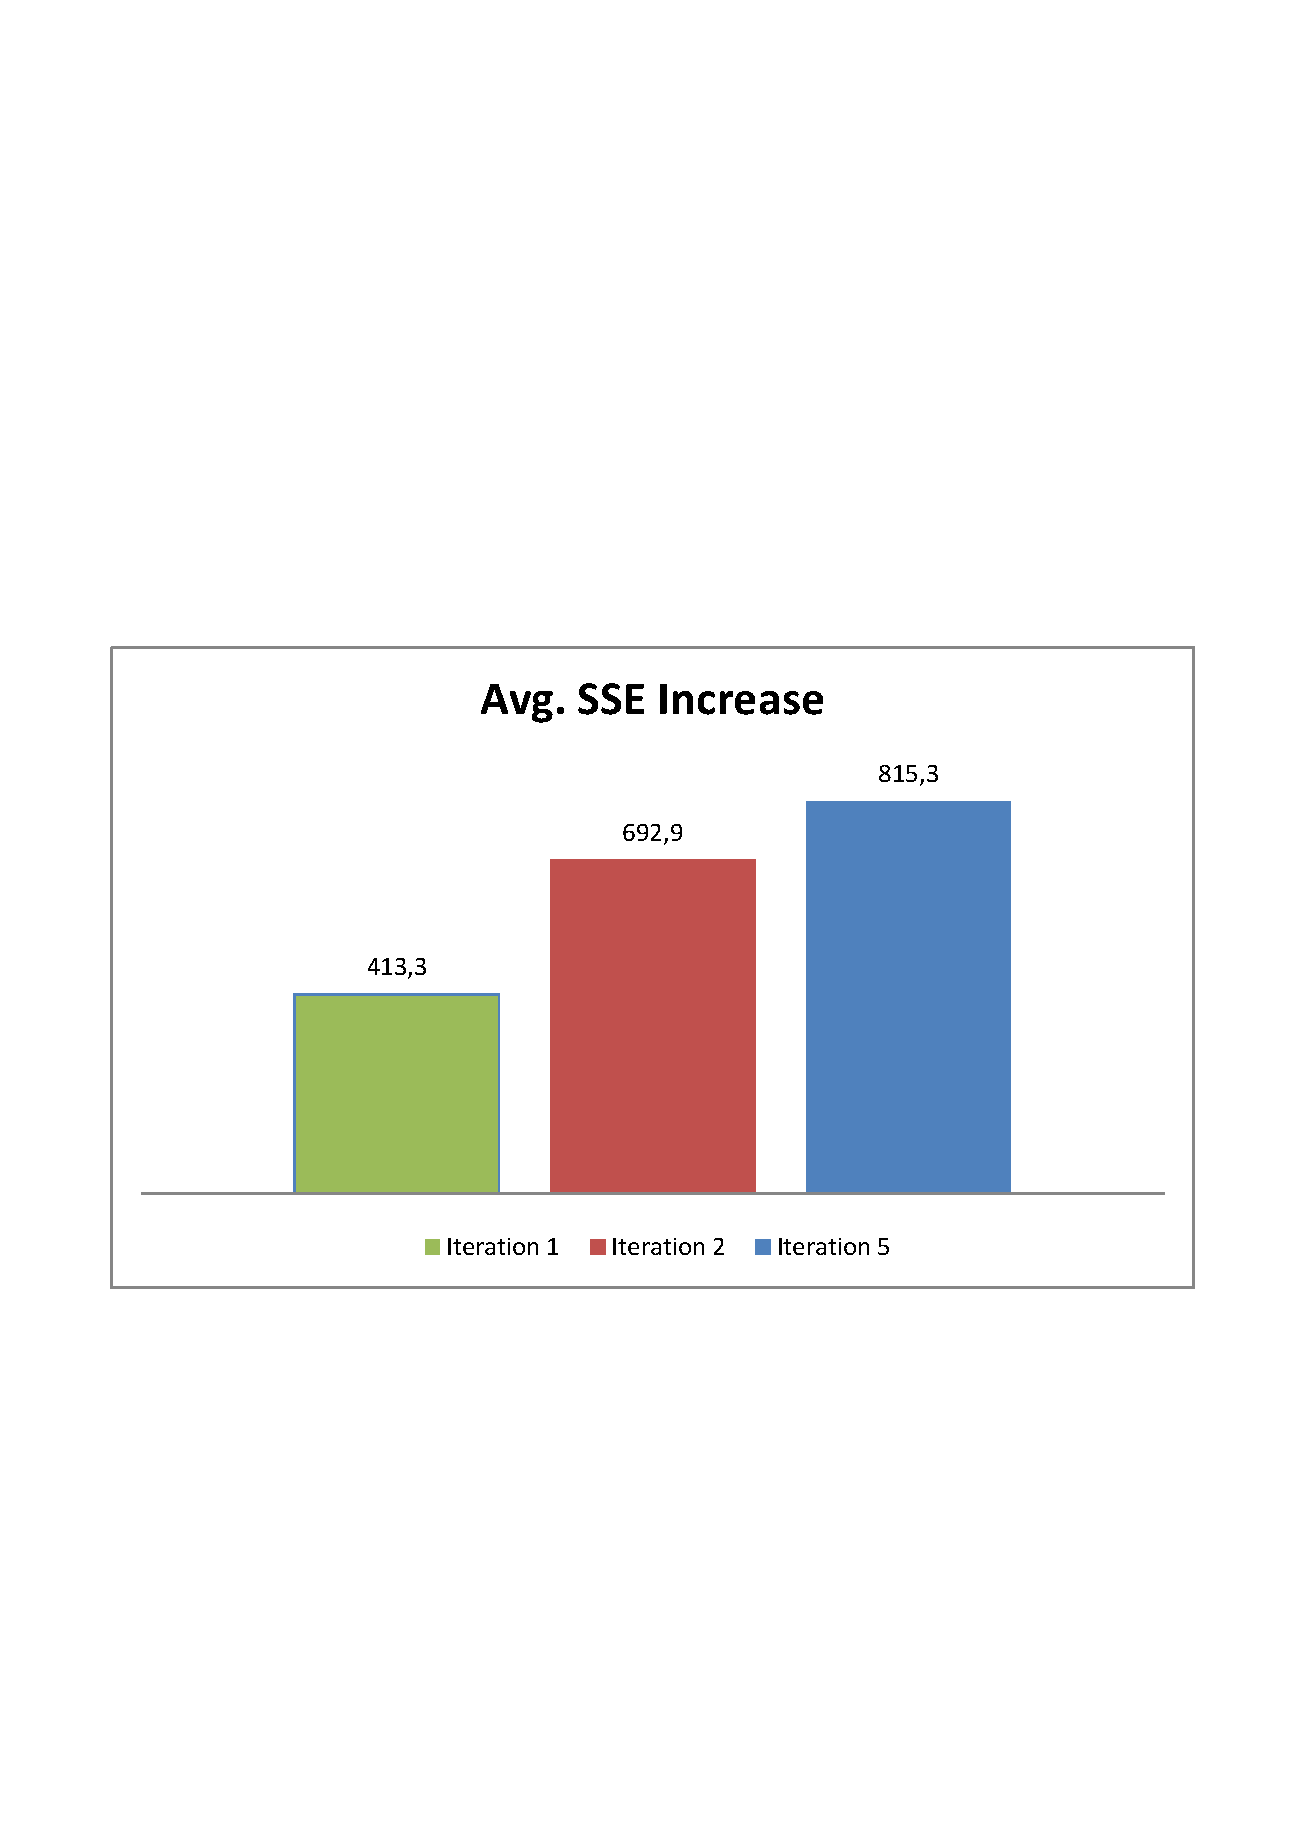
\includegraphics[trim = 10mm 90mm 10mm 100mm, clip, width=0.75\textwidth]{Figures/experiments/zdataWO_AvgSSEIncrease.pdf}
\caption{This figure shows the average aggregated SSE error between two data batches, for all test runs.}
\label{fig:AvgSSEIncrease}
\end{figure}

\newpage

\section{Cluster Quality - Generated Dataset}
In the second cluster quality experiment a generated dataset is used. This dataset is generated with three normal distributions that changes and move from each other in the course of ten data batches. The idea is to measure the SSE error when facing a rapid changing data, in that sense that the distributions are moving between chunks of data. 

Finding a method that can represent a stable SSE error and a downward trend is of high value, as explained in the Section~\ref{sec:cq_realdataset}. The Figure~\ref{fig:results_gen_AvgSSEEachDataBatch} shows the SSE error that was measured on average for all the ten test runs when clustering the ten data batches.

\begin{figure}[ht]
\centering
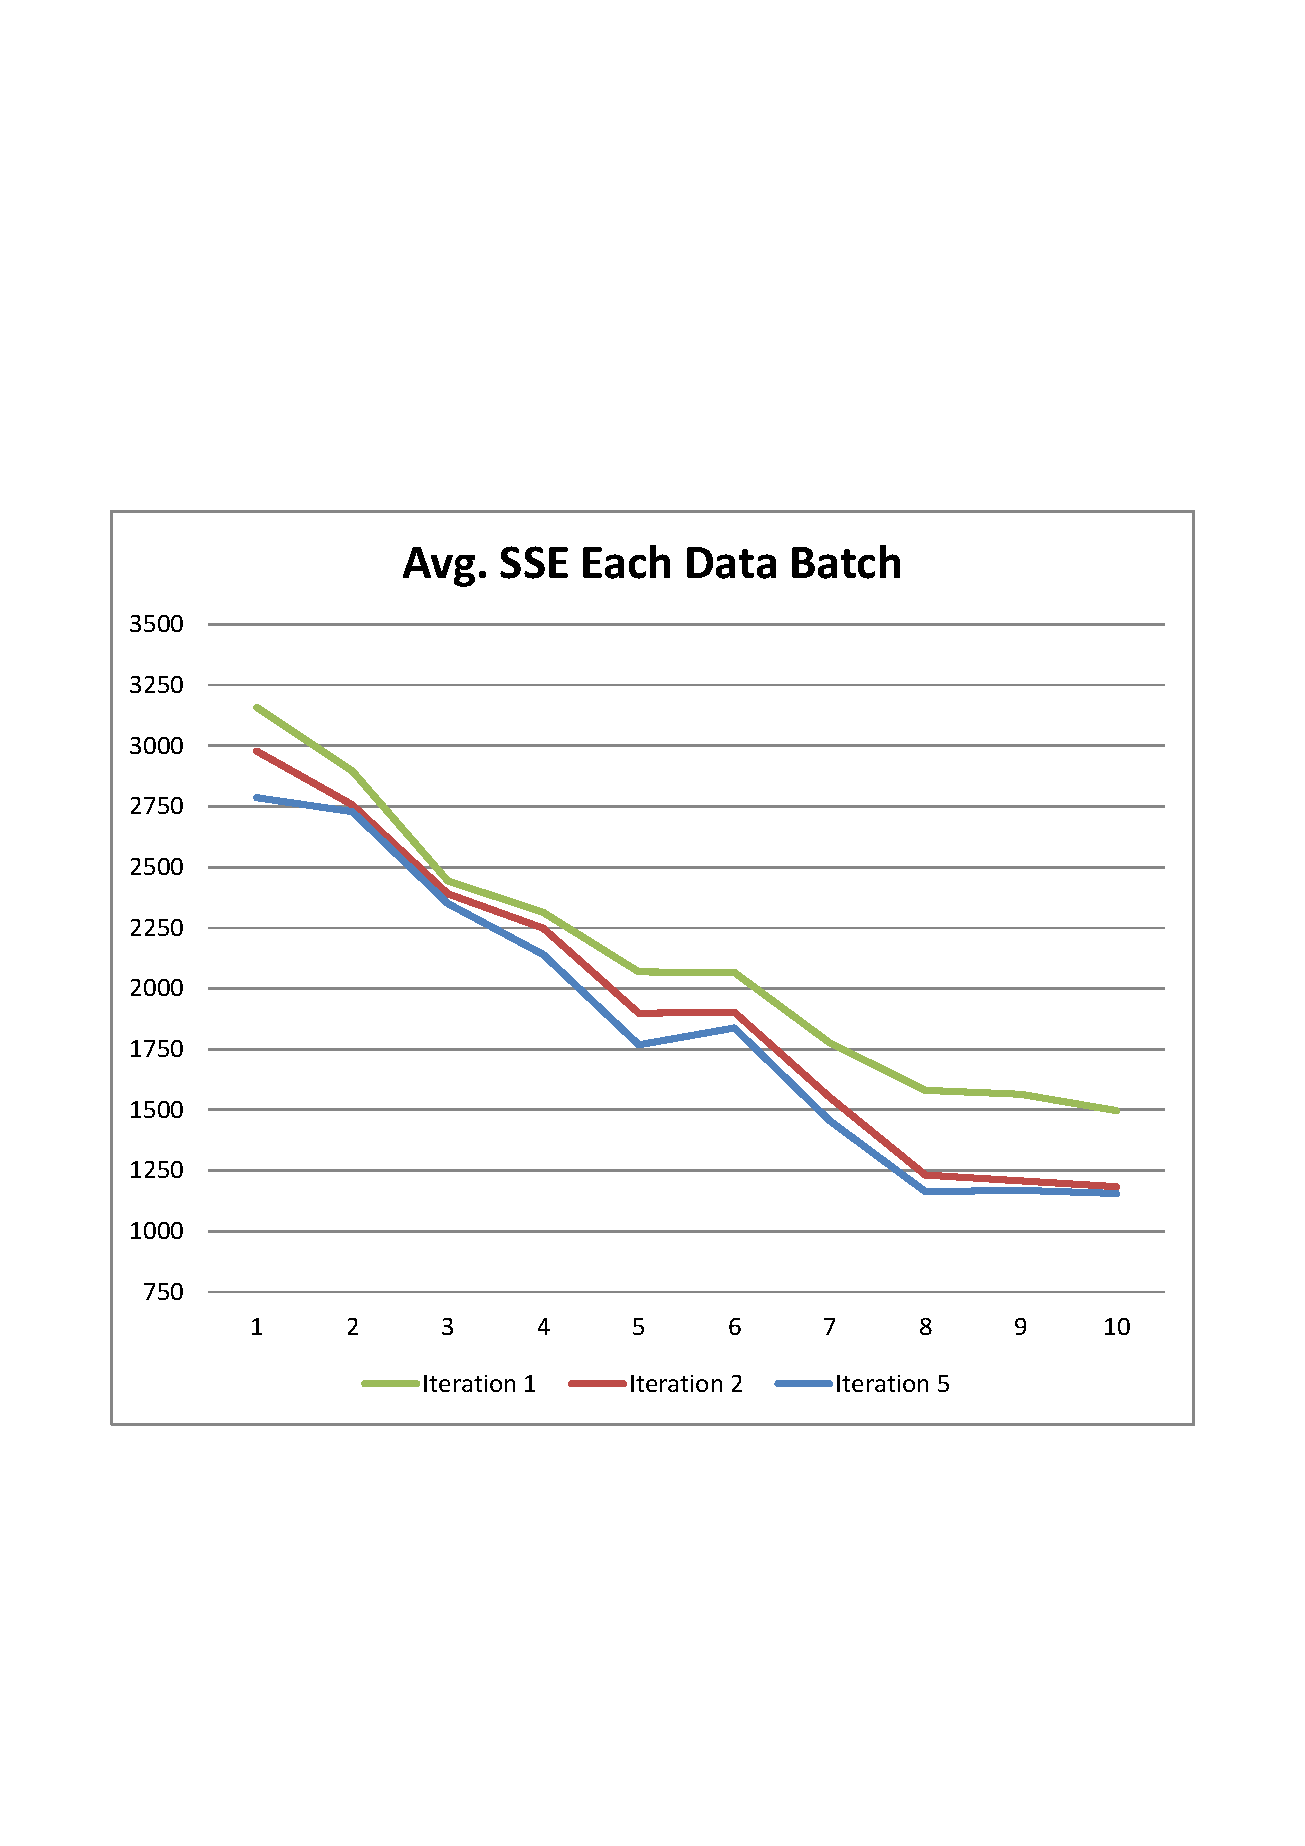
\includegraphics[trim = 10mm 70mm 10mm 80mm, clip, width=0.75\textwidth]{Figures/experiments/gen_AvgSSEEachDataBatch.pdf}
\caption{This figure compares the average SSE error after clustering each generated data batch, using the three different $n$-iterations methods. }
\label{fig:results_gen_AvgSSEEachDataBatch}
\end{figure}

We can see that both the \textit{Iteration 1} and \textit{Iterantion 2} methods show a downward trend for the SSE error but the \textit{Iteration 5} method is taking a relatively big step from data batch $5$ to $6$. Methods \textit{Iteration 2} and \textit{Iteration 3} show the lowest SSE error for the last data batch, in Table~\ref{tab:results_gen_avgSSEeachDataBatch}, with only $2.36\%$ difference, and there is large gap of $22.78\%$ between \textit{Iteration 1} and \textit{Iteration 5}.

\begin{table}[h]
\centering
\begin{tabular}{| l | r | r |}
    \hline
    & \textit{Iteration 2} & \textit{Iteration 5} \\ \hline
    \textit{Iteration 1} & $20.91\%$ & $22.78\%$  \\ \hline
    \textit{Iteration 2} & & $2.36\%$ \\ \hline
\end{tabular}
\caption{This table shows the average SSE error difference on the last generated data batch, between the three methods.}
\label{tab:results_gen_avgSSEeachDataBatch}
\end{table}

This large gap between \textit{Iteration 1} and the other methods is because in this dataset the three distributions are changing relatively fast, moving it in a determined direction in each data batch. Making it hard to keep up with the changes with $1$-iteration while the other methods are moving closer to each next data batch.

In Figure~\ref{fig:results_gen_AvgIncreaseEachTestRun} we can see the measured SSE error when it increases between data batches, e.g. where a SSE error for a batch is higher than the previous data batch. The \textit{Iteration 2} method is now showing the lowest error on average, and in $4$ out of $10$ tests it almost doesn't increase the SSE. Method \textit{Iteration 5} is however very interesting in test $3$ where it much lower than the other methods. 

\begin{figure}[ht]
\centering
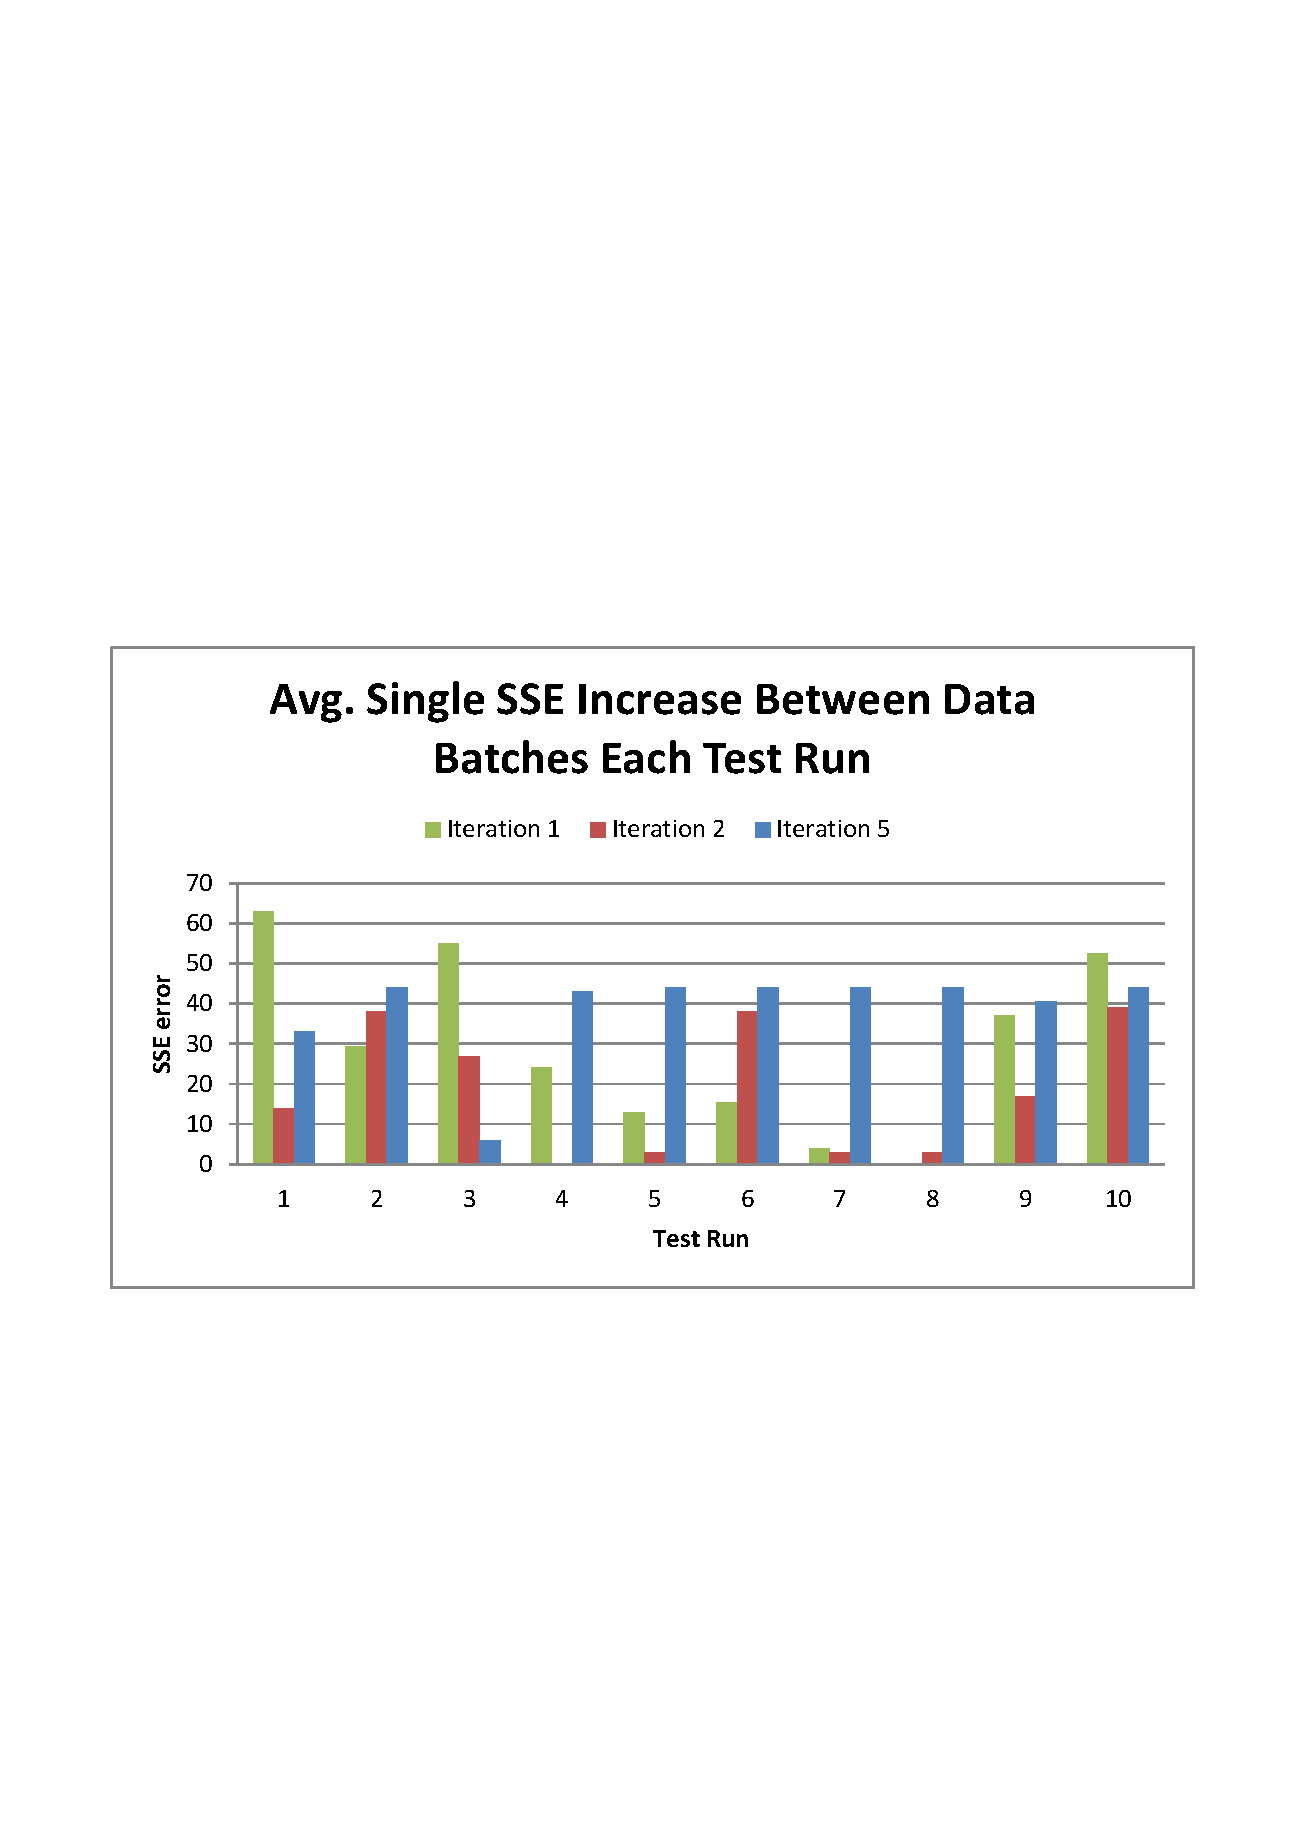
\includegraphics[trim = 10mm 90mm 10mm 100mm, clip, width=0.75\textwidth]{Figures/experiments/gen_AvgSingleSSEIncreaseBetweenDataBatchesEachTestRun.pdf}
\caption{Here we can see on average the single SSE error increase that was measured, when SSE increases from one batch to another. }
\label{fig:results_gen_AvgIncreaseEachTestRun}
\end{figure}

Looking into the data it shows that the \textit{Iteration 5} method manages to report much lower SSE error than the other methods when processing data batch number 6, using the centroids found in data batch number 5. And in general all the methods had a SSE increase when processing batch 6, see Figure~\ref{fig:results_gen_DifficultDataBatches} which data batches gave problems over all the tests. Batch 6, 9 and 10 gave high SSE increase on average, but the batch 6 had the far most error for all the methods. 

\begin{figure}[ht]
\centering
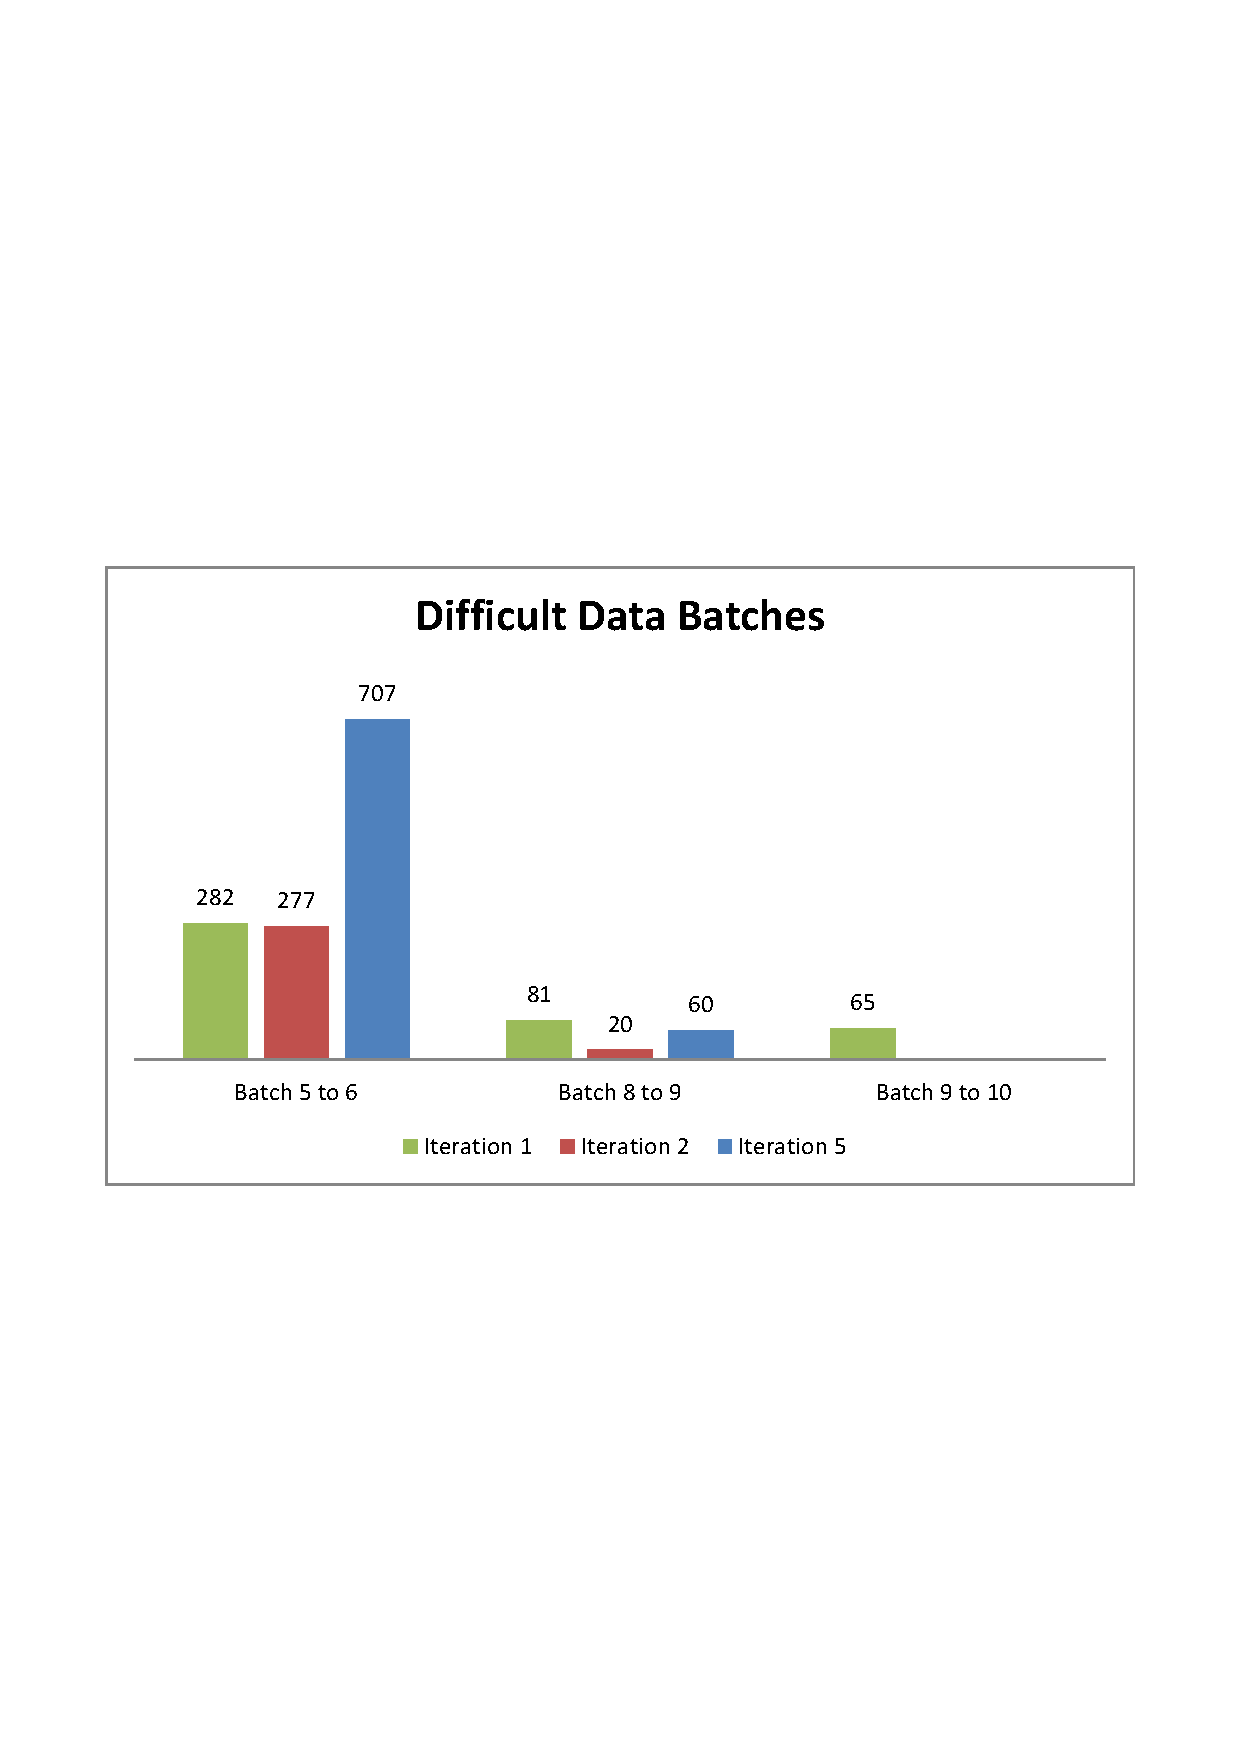
\includegraphics[trim = 10mm 90mm 10mm 95mm, clip, width=0.75\textwidth]{Figures/experiments/gen_DifficultDataBatches.pdf}
\caption{This figure shows the data batches where all methods increased the SSE error going from one data batch to the next. }
\label{fig:results_gen_DifficultDataBatches}
\end{figure}

When looking at the data population for data batch 5 and 6 we can see that there is a clear change in the data, going from batch 5 to 6, see Figure~\ref{fig:results_gensubfigures}. The figure on to the right shows clearly that one of the clusters have disconnected from the rest, and this seems to give problems for all methods. \textit{Iteration 5} had the most troubles with batch 6 in general, most likely by moving its centroids to aggressively through many iterations and end up in a local optimum.



\begin{figure}[ht!]
        \begin{center}
        \subfigure{%
            \label{fig:first}
            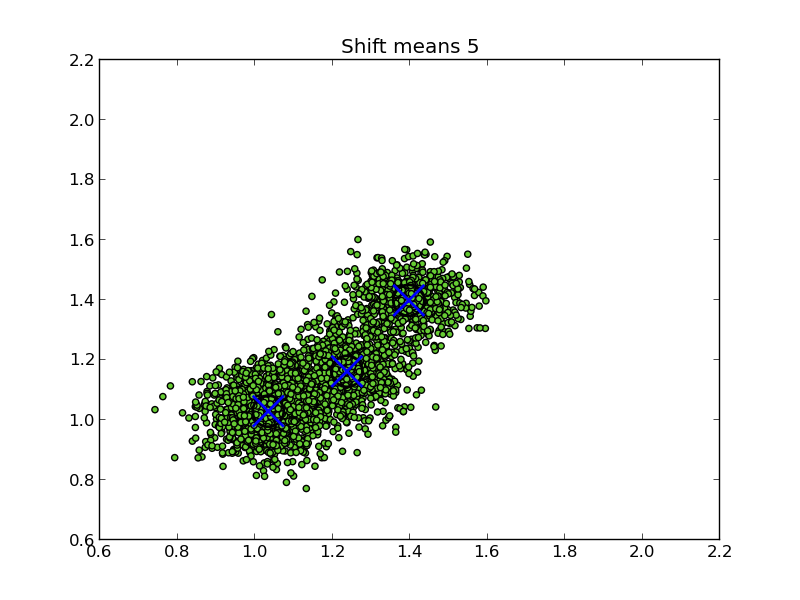
\includegraphics[width=0.5\linewidth]{Figures/gmeans/4_genshiftmeans.png}
        }%
        \subfigure{%
           \label{fig:second}
           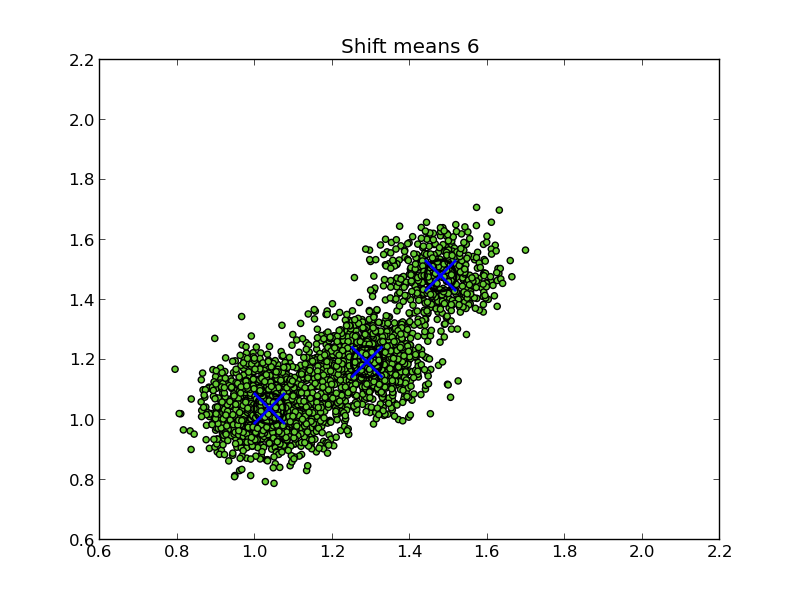
\includegraphics[width=0.5\linewidth]{Figures/gmeans/5_genshiftmeans.png}
        } %  ------- End of the first row ----------------------%
        \end{center}
    \caption{These figures shows how the data distribution changes from data batch 5 to 6. In the right figure we can see a cluster that has moved from the other two clusters.}
   \label{fig:results_gensubfigures}
\end{figure}

For the \textit{Iteration 5} method from test 3 in Figure~\ref{fig:results_gen_AvgIncreaseEachTestRun}, it is likely that the random initial centroids for the first batch, leads the centroids very close to the highest population such that it didn't fell in to a trap when processing batch number 6, thus measuring low SSE for that method. The same happens in general for the other methods since they move much slower and are closer to the main population.

Looking at the measured SSE error that happened between all sets of data batches, we can see in Figure~\ref{fig:results_gen_TotalSSEIncreaseEachTestRun} that \textit{Iteration 2} is reporting over all tests very low SSE increase but is high in tests 2, 6 and 10, which were related to the data batch number 6, discussed above.

\begin{figure}[ht]
\centering
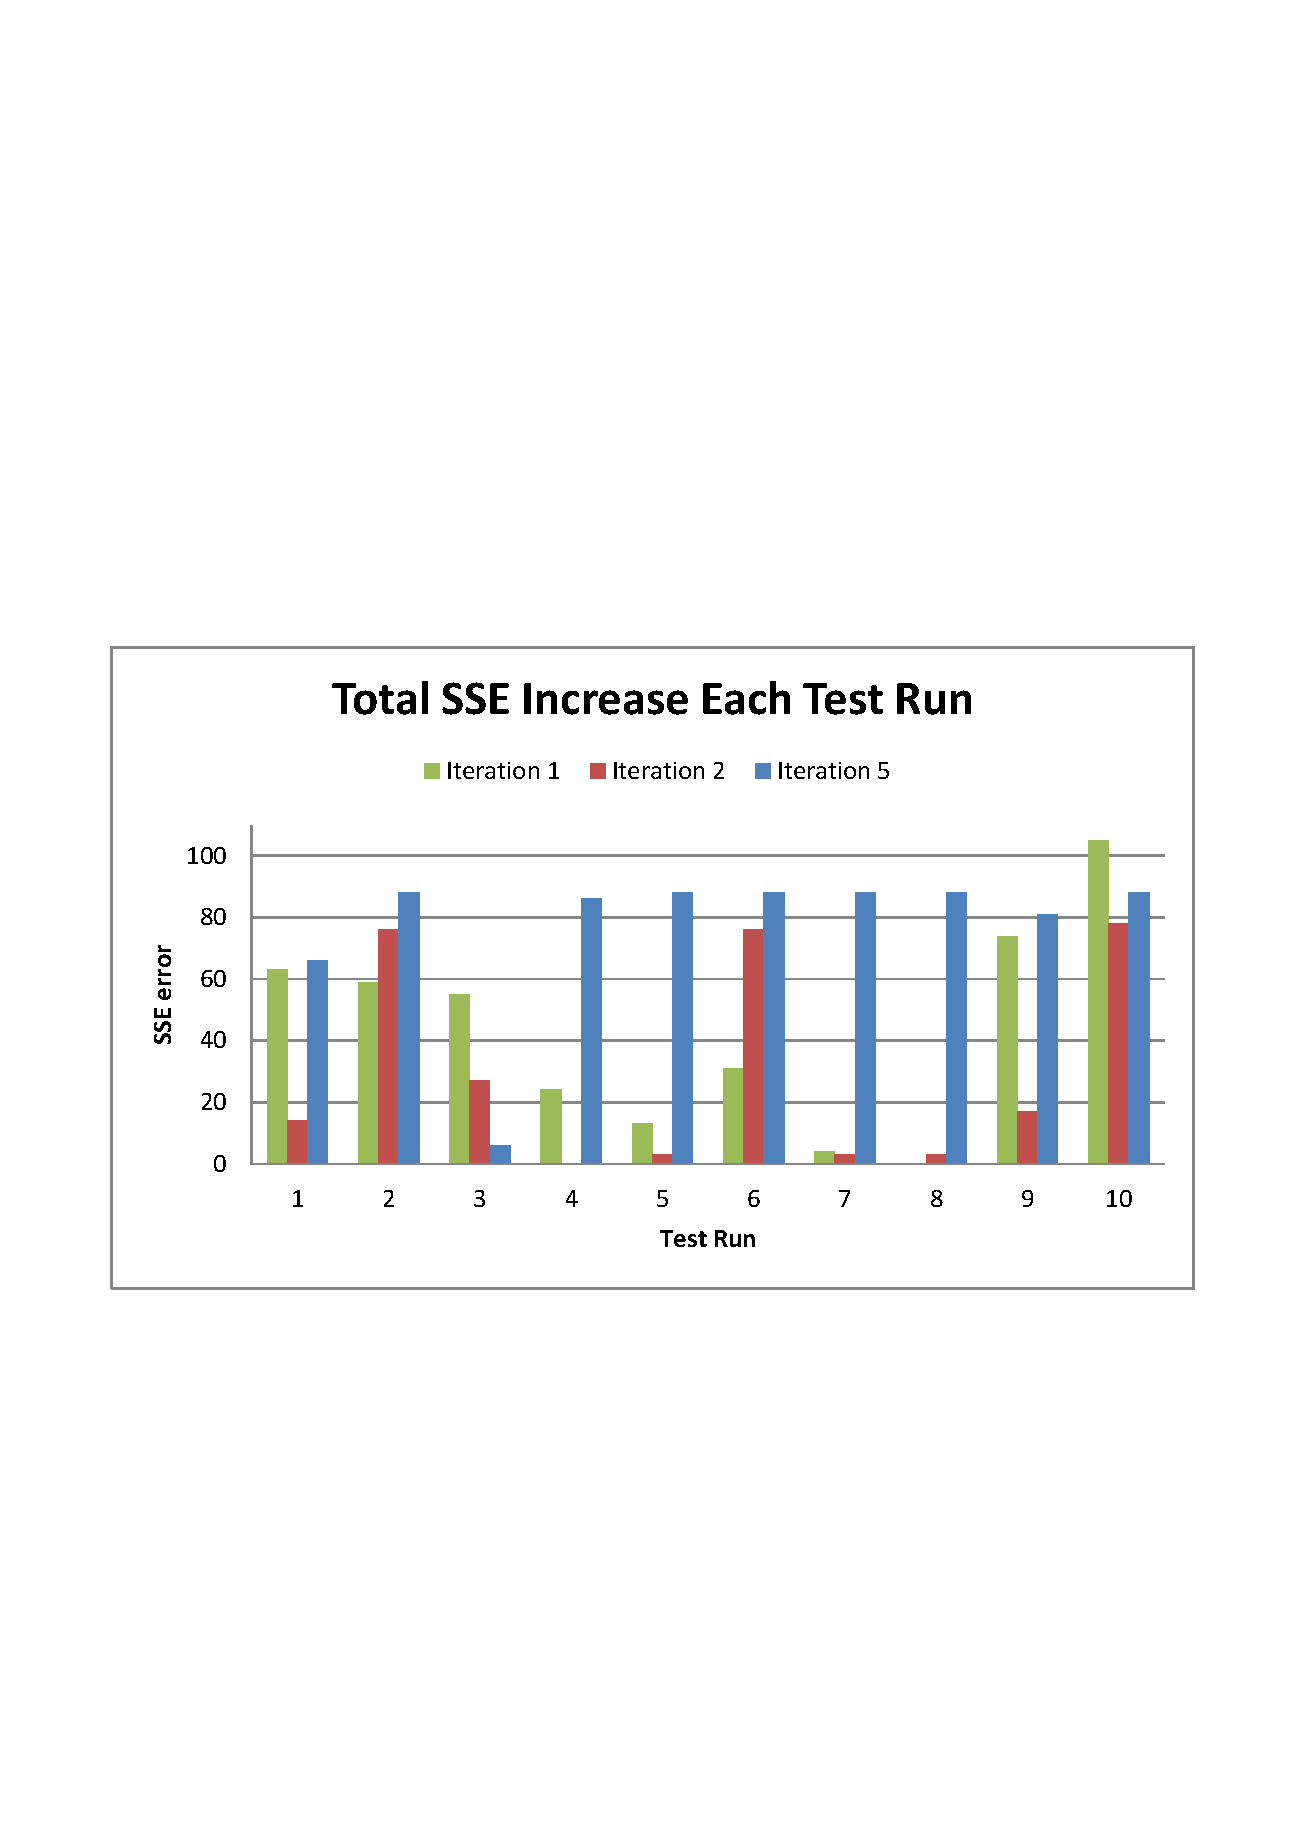
\includegraphics[trim = 10mm 90mm 10mm 100mm, clip, width=0.75\textwidth]{Figures/experiments/gen_TotalSSEIncreaseEachTestRun.pdf}
\caption{This figure shows the aggregated SSE error between two data batches for each test run.}
\label{fig:results_gen_TotalSSEIncreaseEachTestRun}
\end{figure}

When aggregating all the SSE error between all the sets of data batches over all runs we get \textit{Iteration 2} with the lowest average, with \textit{Iteration 1} not far away.

\begin{figure}[ht]
\centering
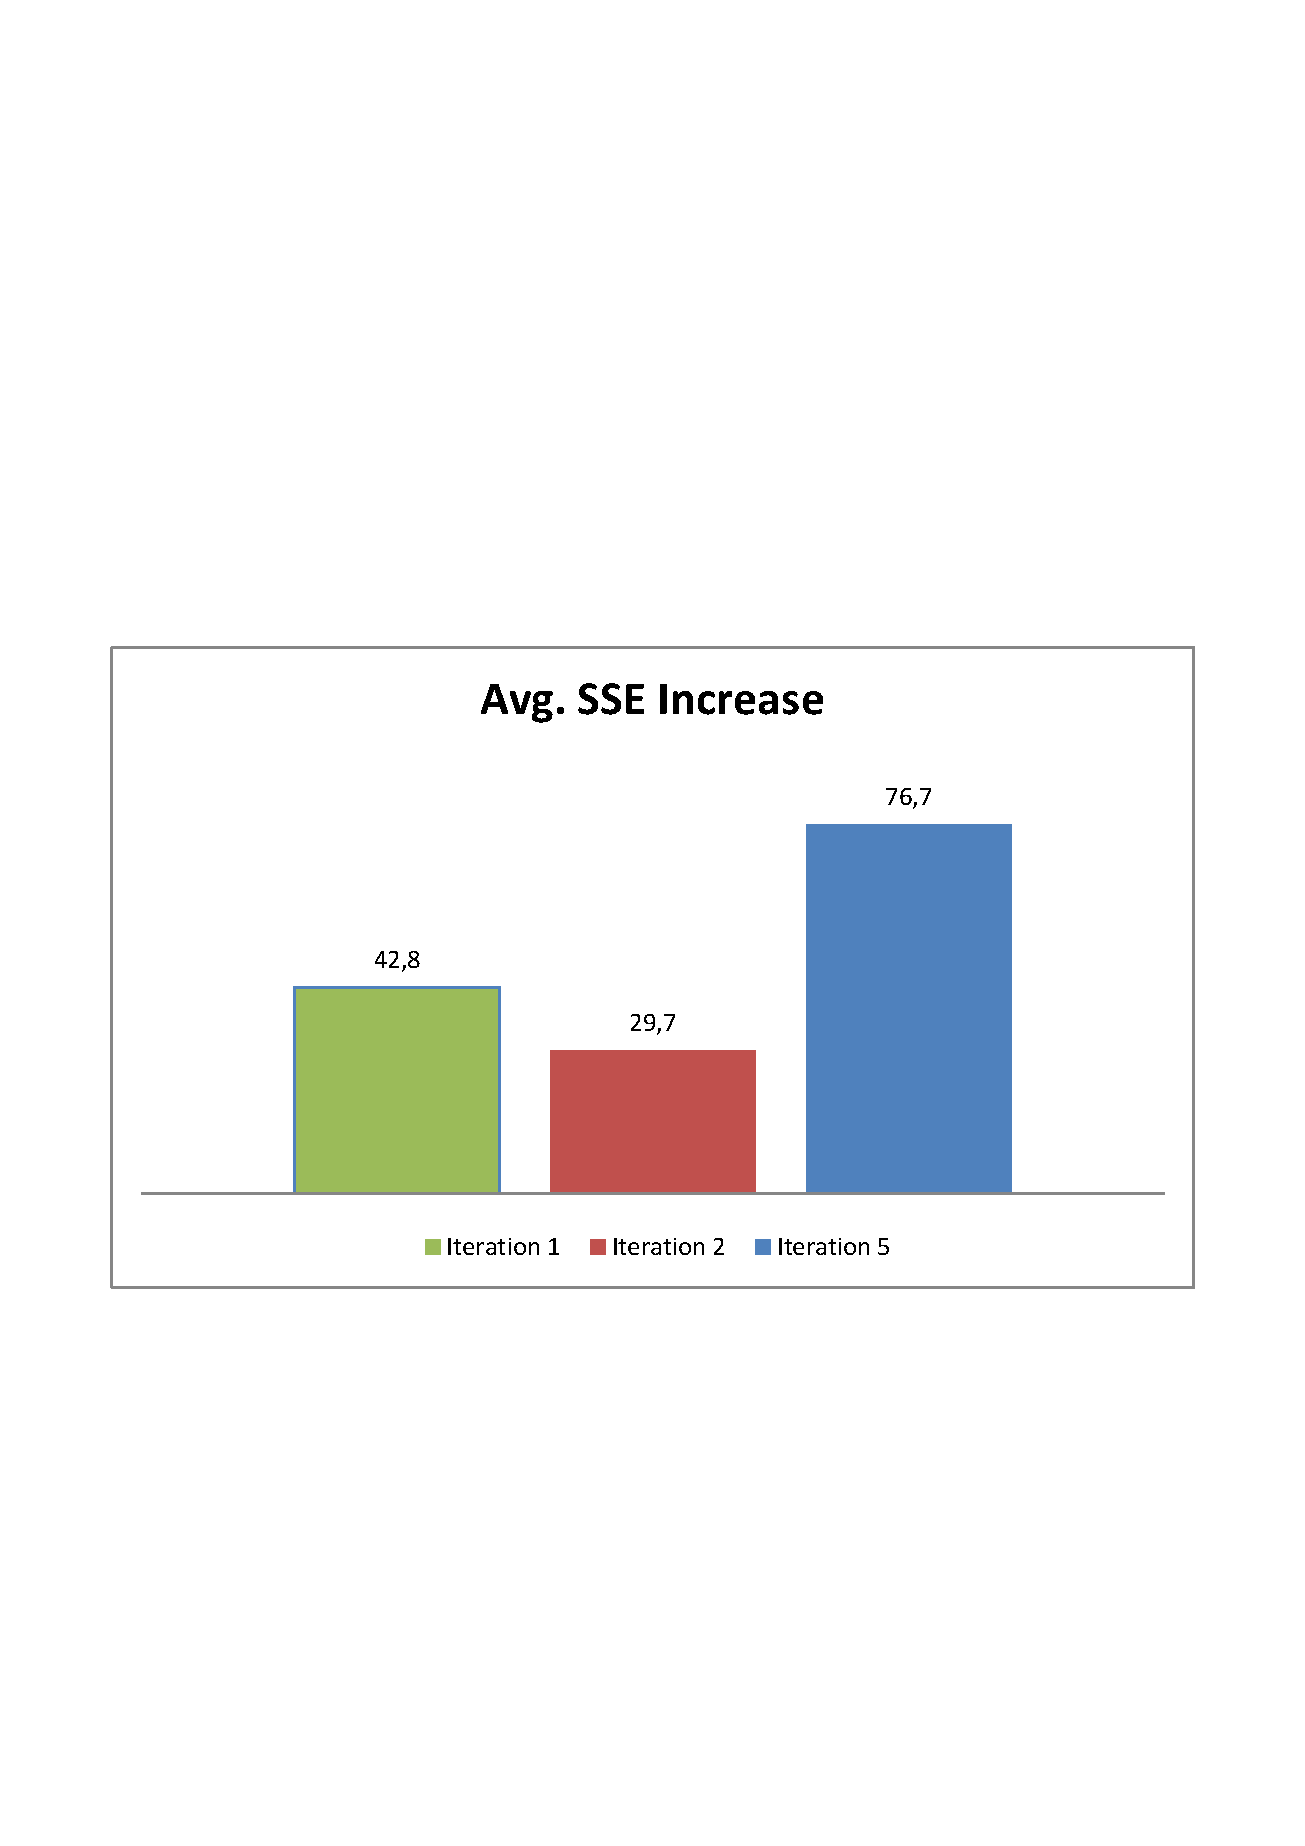
\includegraphics[trim = 10mm 90mm 10mm 100mm, clip, width=0.75\textwidth]{Figures/experiments/gen_AvgSSEIncrease.pdf}
\caption{This figure shows the average aggregated SSE error between two data batches, for all test runs. }
\label{fig:results_gen_AvgSSEIncrease}
\end{figure}

\newpage
\section{General Player Behaviour}
The results from real game data cluster quality experiment in Section~\ref{sec:cq_realdataset} were used and interpreted to find the general player behaviour. The centroids from the last data batch when using the \textit{Iteration 1} method was used as basis for this experiment, from the test run that had the the lowest SSE. 

The three centroids from the final data batch, found by the MR k-means algorithm, describes the average behaviour of the three clusters found, after clustering incrementally the ten data batches. See Table~\ref{tab:results_centroids} for the centroids and their z-score values, and Figure~\ref{fig:results_zscoredataset} for the visualization of the clusters found.

\begin{table}[h]
\centering
\begin{tabular}{| l | r | r | r |}
    \hline
    & \textit{Logins} & \textit{Battles} & \textit{Premium spent} \\ \hline
    Centroid 1 & $2.25$ & $1.35$ & $0.06$  \\ \hline
    Centroid 2 & $-0.29$ & $-0.33$ & $-0.31$  \\ \hline
    Centroid 3 & $0.24$ & $1.46$ & $2.62$ \\ \hline
\end{tabular}
\caption{This tables shows the how the final centroids in \textit{z-score} values looked like after clustering the final game data batch file, using the \textit{Iteration 1} method.}
\label{tab:results_centroids}
\end{table}


\begin{figure}[here]
\centerline{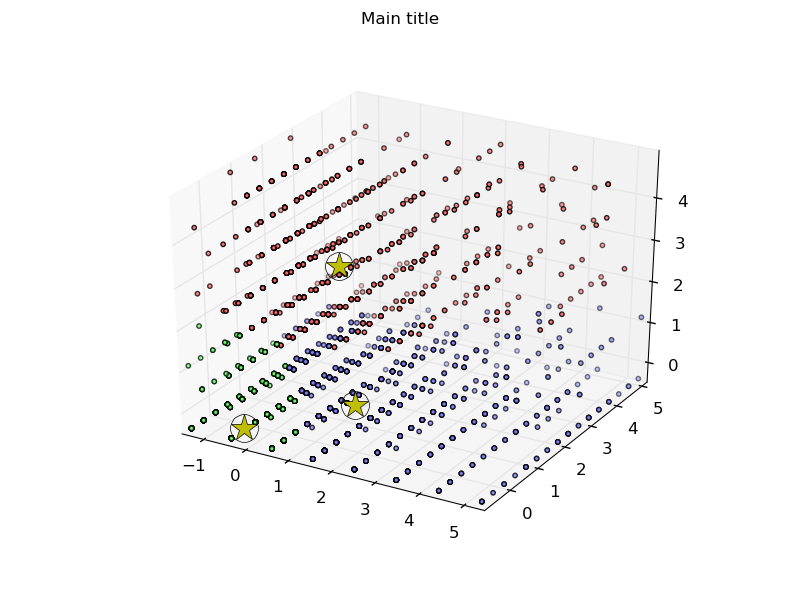
\includegraphics[trim = 10mm 10mm 10mm 20mm, clip, width=0.75\textwidth]{Figures/experiments/zscoreResultsGamedatasetwooutliers.png}}
\caption{This figures shows how the clusters looked like for the final data batch, the centroids are marked with stars.}
\label{fig:results_zscoredataset}
\end{figure}


These standardized values were transformed to their original values as explained in the experiment set-up in Section~\ref{sec:experiment_gpb}. For the original values see Table~\ref{tab:results_centroidsoriginalvalues}. The centroids represent the general player behaviour based on the behavioural features that were used, and can be used to describe behavioural profiles that is found in the data. See Table~\ref{tab:results_playerprofiles} for the player profiles that were extracted and interpreted from the centroids. The profile titles and their descriptions were made from a guess and intuition.

\begin{table}[h]
\centering
\begin{tabular}{| l | r | r | r |}
    \hline
    & \textit{Logins} & \textit{Battles} & \textit{Premium spent} \\ \hline
    Centroid 1 & $3.80$ & $2.86$ & $1.51$  \\ \hline
    Centroid 2 & $1.14$ & $1.10$ & $1.12$  \\ \hline
    Centroid 3 & $1.70$ & $2.97$ & $4.19$ \\ \hline
\end{tabular}
\caption{This tables shows the centroids in the original range of values for each game metric, used for interpretability.}
\label{tab:results_centroidsoriginalvalues}
\end{table}

\begin{table}[h]
\centering
\begin{tabular}{| l | r | l | l |}
    \hline
    \textit{Profile title} & \textit{\% of P} & \textit{Description} \\ \hline
    Active Joe & $9.39\%$ & Explores areas and fights battles \\ \hline
    Lazy & $81.12\%$ &  Jumps in and out of the game \\ \hline
    Golden Warrior & $9.49\%$ & Fights battles and spends in-game money \\ \hline
\end{tabular}
\caption{This table shows the player profiles and their size in the player population. Extracted from the centroids that describe the $k$ average player feature vectors after incrementally clustering multiple batches of game data.}
\label{tab:results_playerprofiles}
\end{table}


\newpage
\section{Scalability}
The results from the scalability experiment shows that the MR k-means algorithm is scalable algorithm that is fully capable to be run on Amazon EMR web service, launching on-demand Amazon Elastic Hadoop clusters. In Figure~\ref{fig:results_scalevertical} we can see the vertical scaling, where the computing power is doubled but processing the same size of data. 

\begin{figure}[ht]
\centering
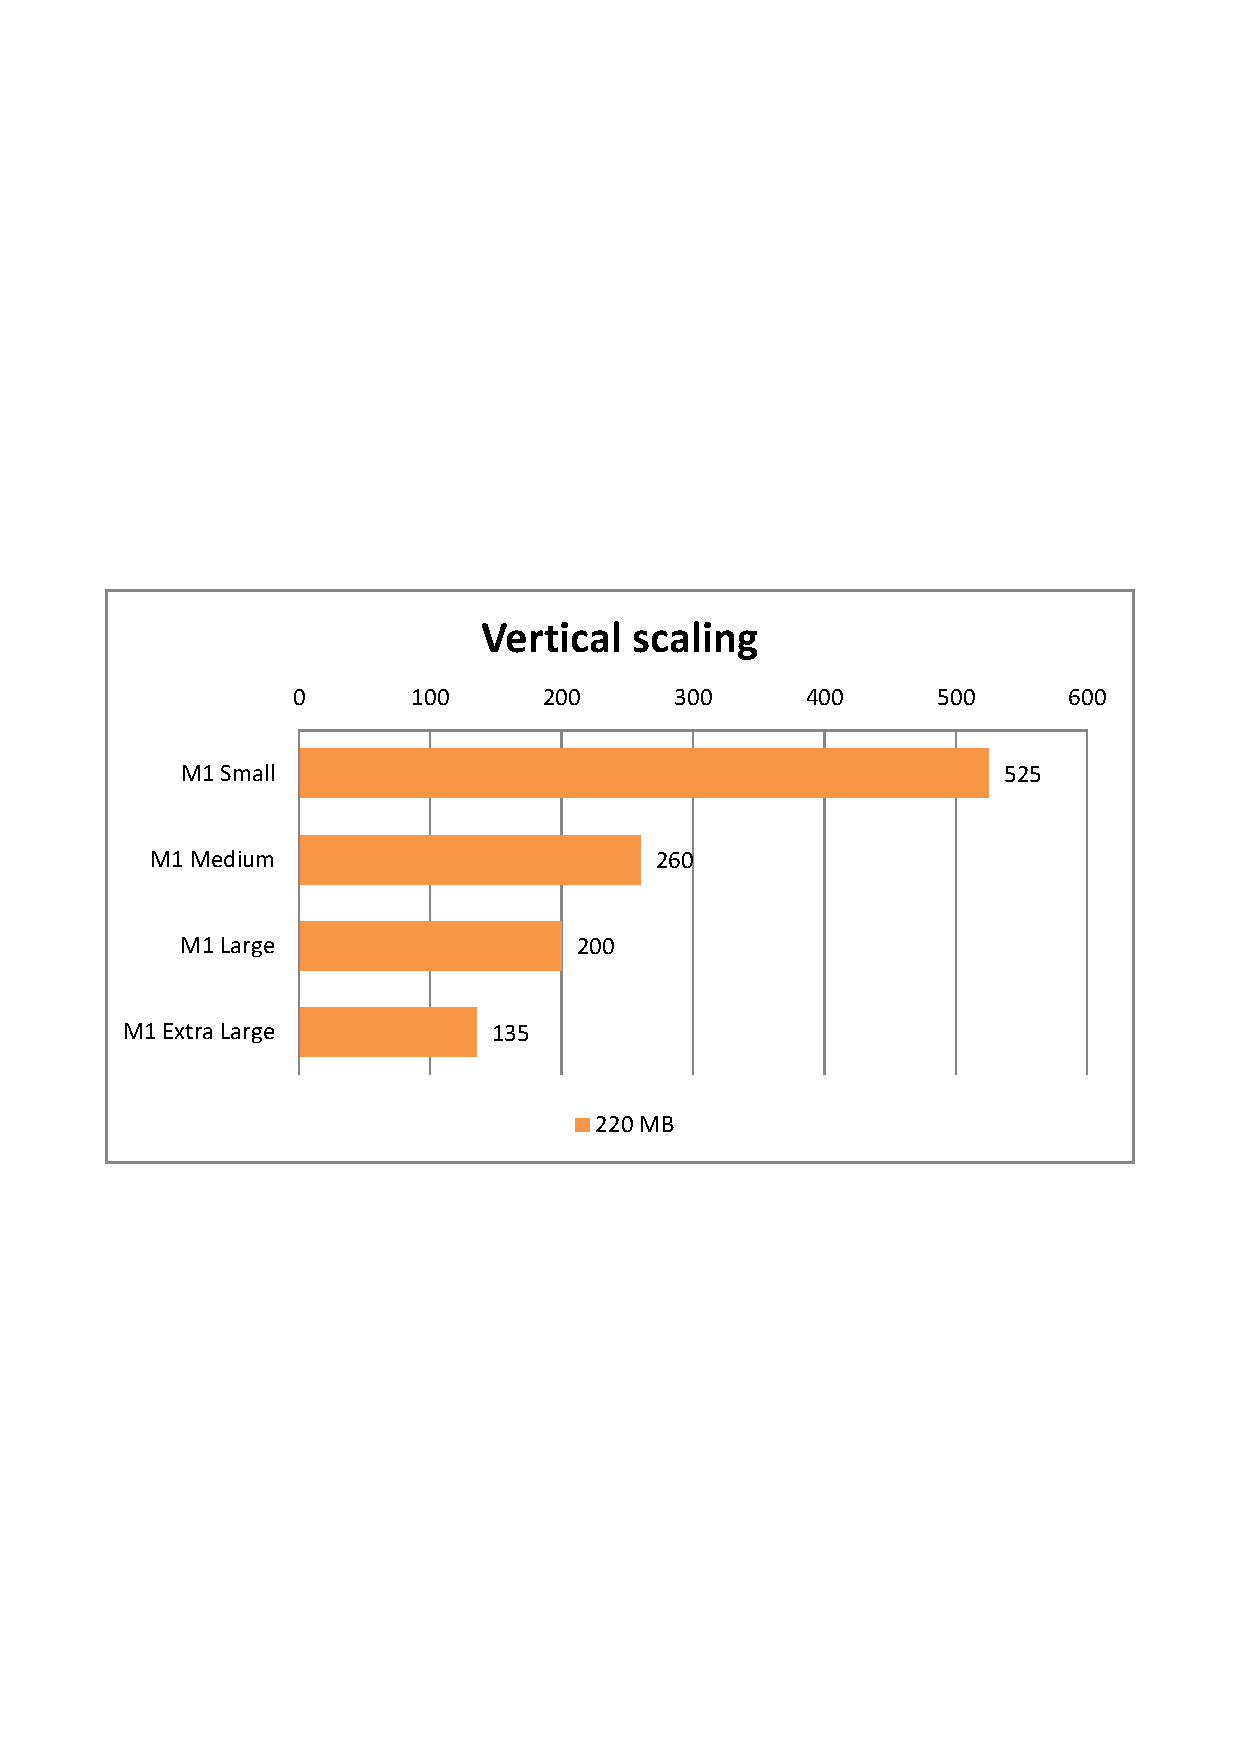
\includegraphics[trim = 10mm 90mm 10mm 90mm, clip, width=0.75\textwidth]{Figures/experiments/scale_vertical.pdf}
\caption{This figure shows the running time (in sec) when doing vertical scaling for the MR k-means algorithm. Doubling the computing power on same dataset size.}
\label{fig:results_scalevertical}
\end{figure}

The horizontal scaling results are in Figure~\ref{fig:results_scalehorizontal}, and show the running time when doubling the number of computers or nodes when clustering the same size of data.  


\begin{figure}[ht]
\centering
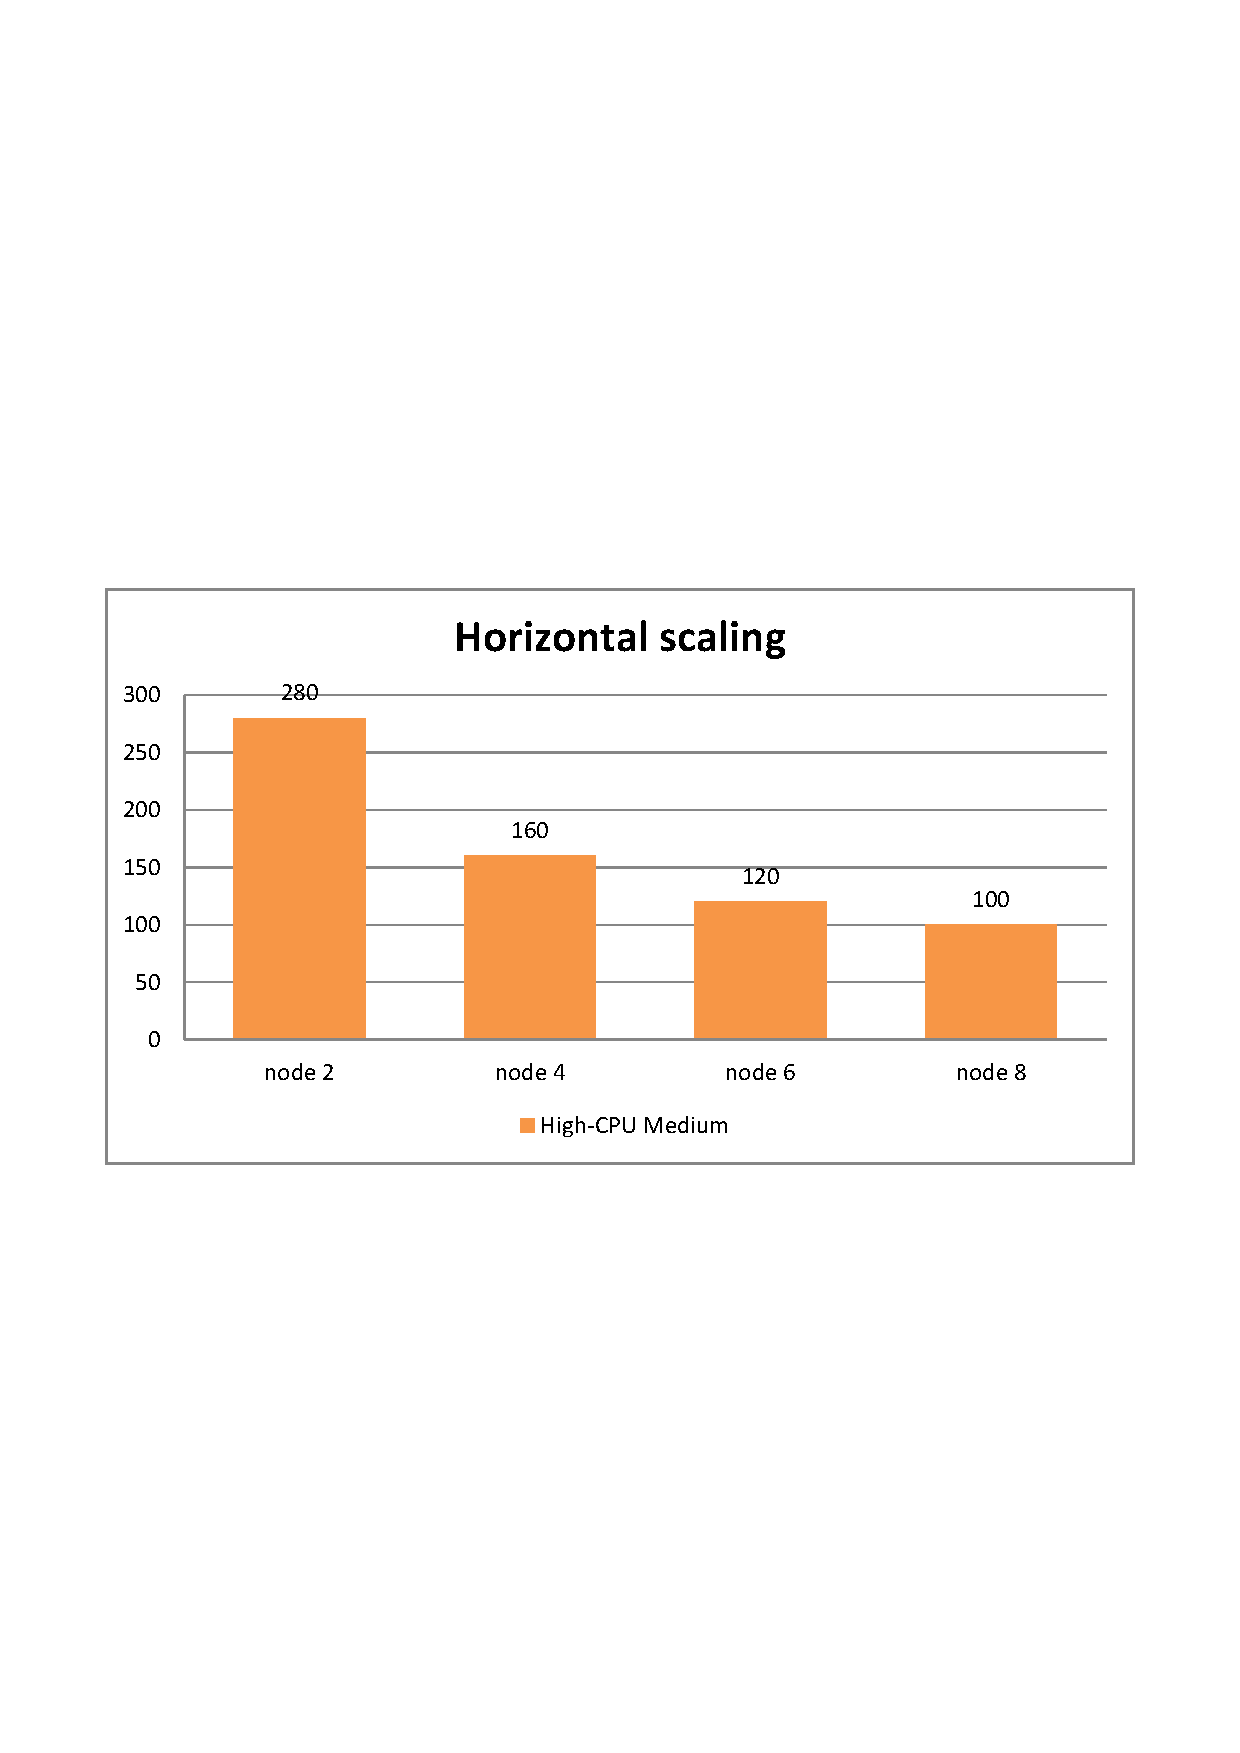
\includegraphics[trim = 10mm 90mm 10mm 90mm, clip, width=0.75\textwidth]{Figures/experiments/scale_horizontal.pdf}
\caption{This figure shows the running time (in sec) when doing a horizontal scaling for the MR k-means algorithm. The number of computer nodes are doubled each time on the same size of data. }
\label{fig:results_scalehorizontal}
\end{figure}

The MR k-means scales both horizontally and vertically, showing the biggest performance jumps when doubling in the beginning of the tests. In Table~\ref{tab:results_scale_scaling} we can see how the MR k-means scales when doubling both the number of computer nodes and dataset sizes, resulting in nearly the same execution time for all tests.

\begin{table}[h]
\centering
\begin{tabular}{| l | l | l |}
    \hline
    \textit{Size} & \textit{\# nodes} & \textit{time in sec} \\ \hline
    220 MB & 2 & 280  \\ \hline
    440 MB & 4 & 280  \\ \hline
    880 MB & 8 & 285 \\ \hline
    1760 MB & 16 & 285 \\ \hline
\end{tabular}
\caption{This table shows the execution time for the MR k-means algorithm when doubling the computer nodes and the dataset size.}
\label{tab:results_scale_scaling}
\end{table}


\newpage
\section{MR K-means Combiner vs. non-Combiner}
Here we look at the running time results the final MR k-means algorithm was compared with it self but with the Combiner function removed from the MapReduce execution flow. The results show that the Combiner is an essential feature when there is a possibility to reduce problems in the Mapper phase, thus minimizing the data traffic and allowing more efficiency in the MapReduce framework, see Figure

\begin{figure}[ht]
\centering
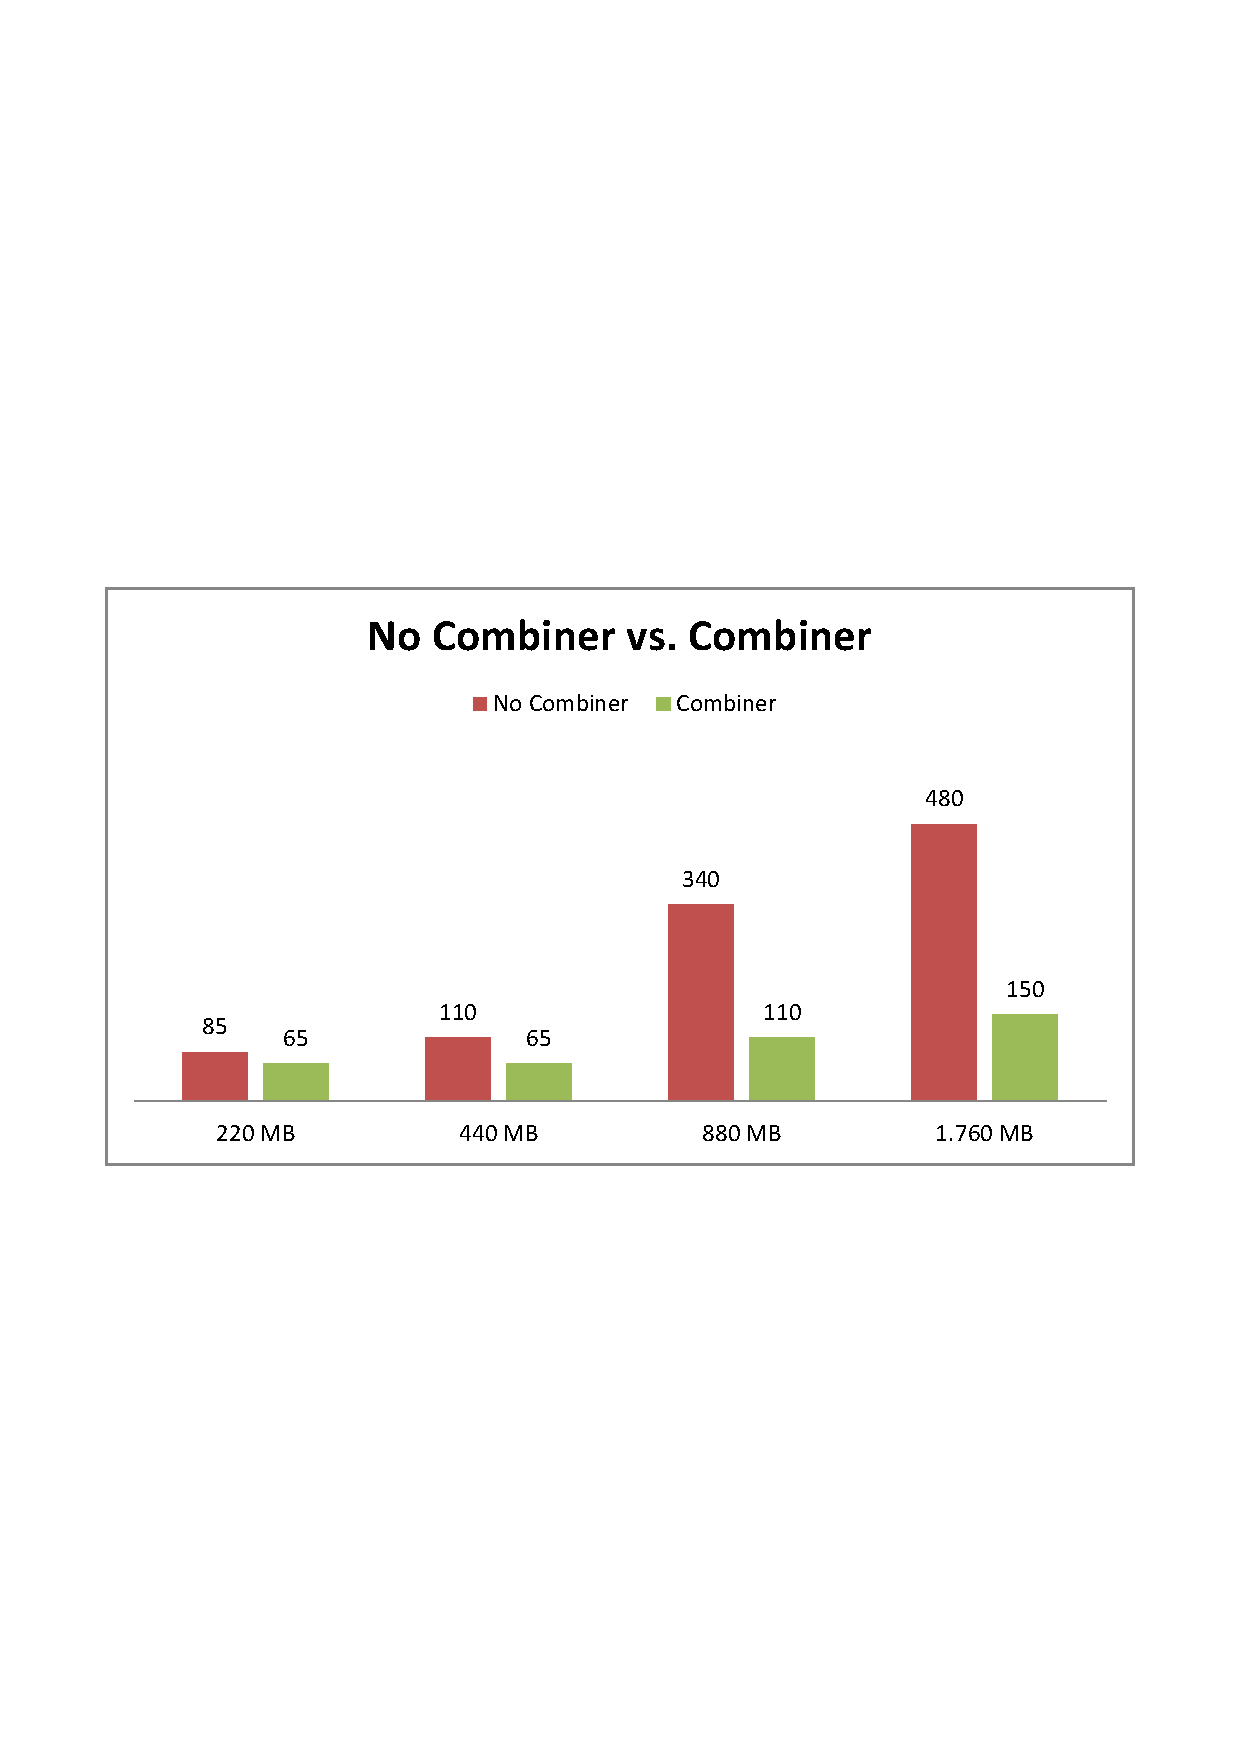
\includegraphics[trim = 10mm 90mm 10mm 90mm, clip, width=0.75\textwidth]{Figures/experiments/combiner.pdf}
\caption{This figure compares the MR k-means algorithm with and without the Combiner function in MR implemented. We can see that having a Combiner can quickly become very efficient versus the non-Combiner version. }
\label{fig:results_combiner}
\end{figure}

\newpage
\section{Nearest Centroid Computation Methods}
The execution time for the three nearest centroid computation methods were compared. The Mapper phase in MapReduce is responsible to find the nearest centroid for each data point, and this computation is the most expensive work when running k-means.

The running time for the naive and the vectorisation versions were compared, leaving the distance matrix implementation out of the picture, for now. See Figure~\ref{fig:results_nearestcentroid} for the comparison of the two. On the figure we can see that the vectorisation version is performing much faster but it converges when running on 8 computer nodes, the MapReduce framework overhead takes over and to make the algorithm run faster we can scale-up by upgrading the computing power.

\begin{figure}[ht]
\centering
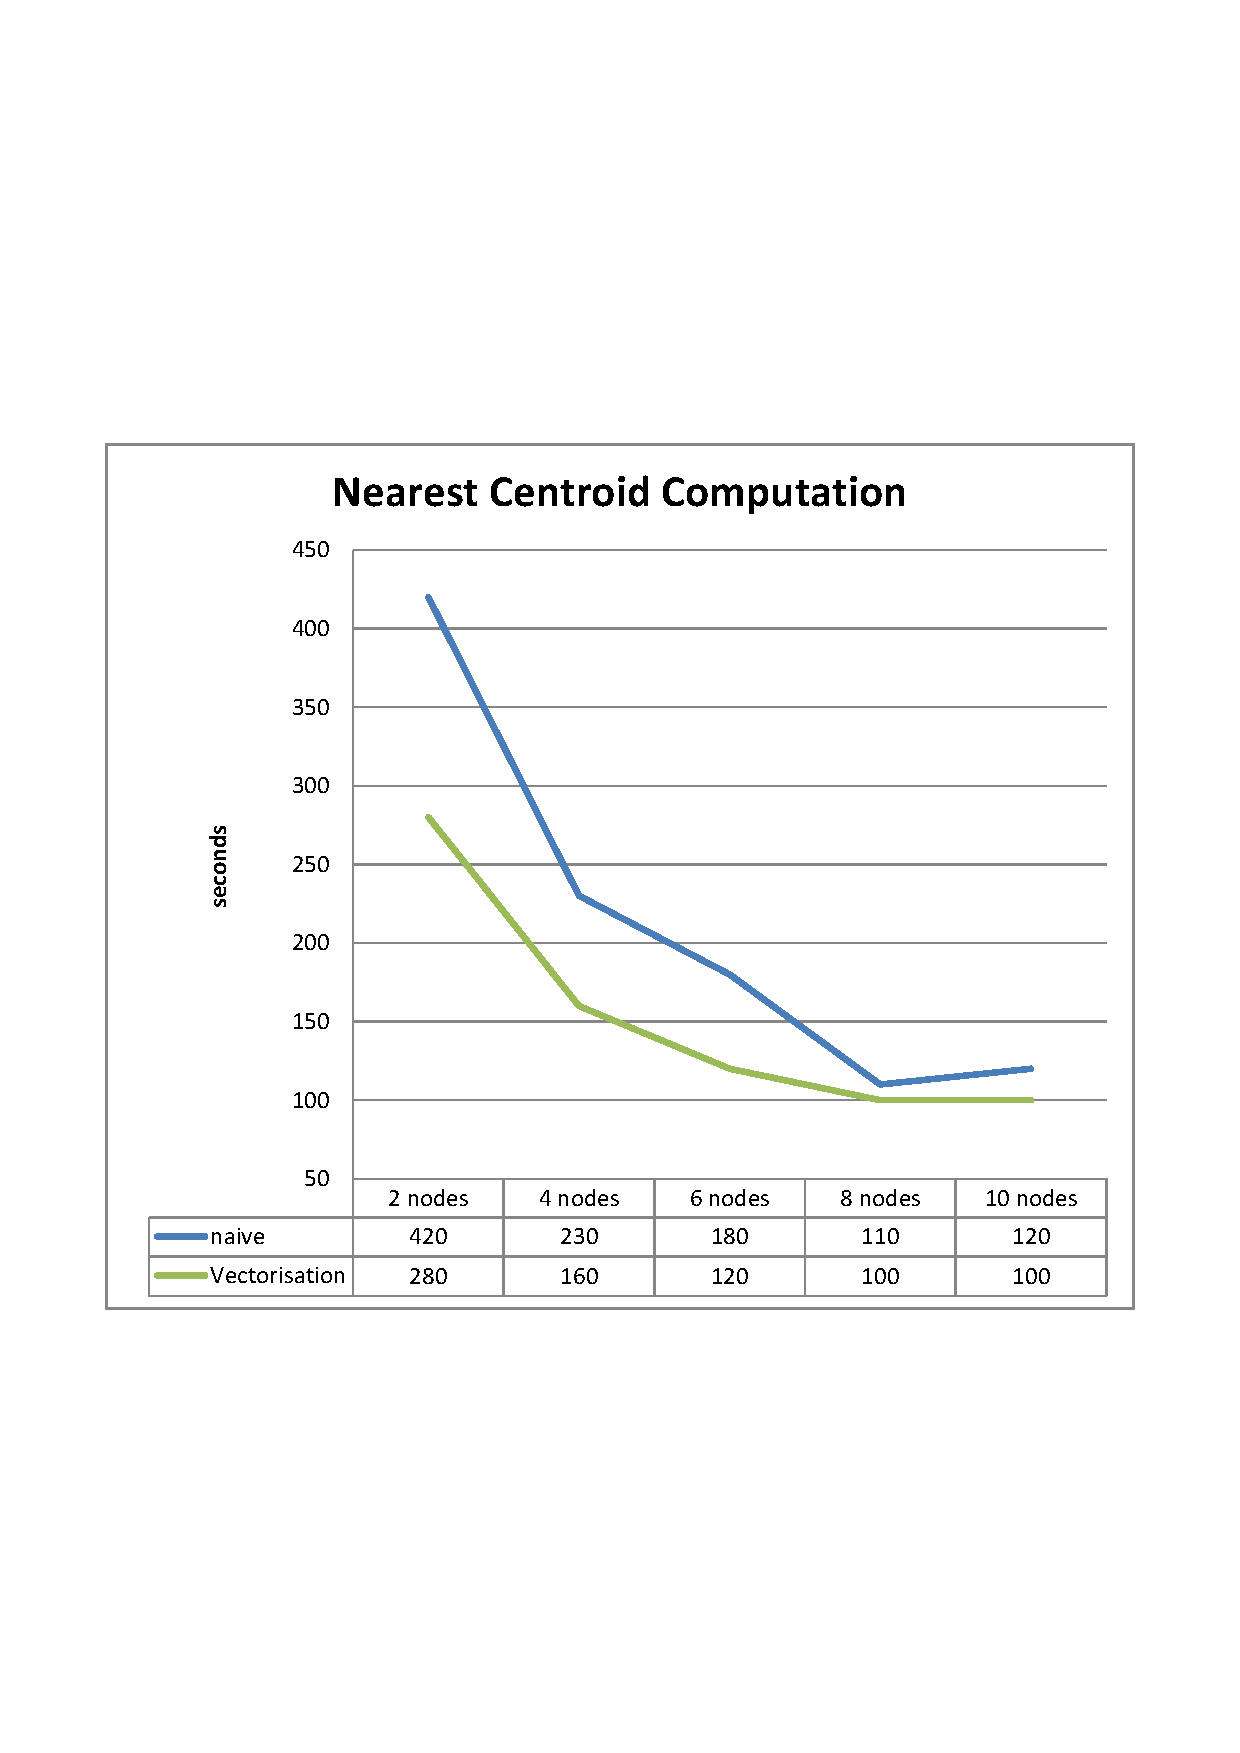
\includegraphics[trim = 10mm 70mm 10mm 70mm, clip, width=0.75\textwidth]{Figures/experiments/nearestcentroid.pdf}
\caption{This figure compares the execution time for the naive and vectorisation methods when computing the nearest centroid.  }
\label{fig:results_nearestcentroid}
\end{figure}

Running the distance matrix version to compute the nearest centroid doesn't work so well on Amazon EMR, compared to the other methods, see Figure~\ref{fig:results_nearestcentroiddist} for the running time for the distance matrix version. Running with 2 nodes resulted in error in the MR execution process and other execution times are much higher, e.g. running with 8 nodes in this setup the distance matrix is $\approx 10$ times slower.

\begin{figure}[ht]
\centering
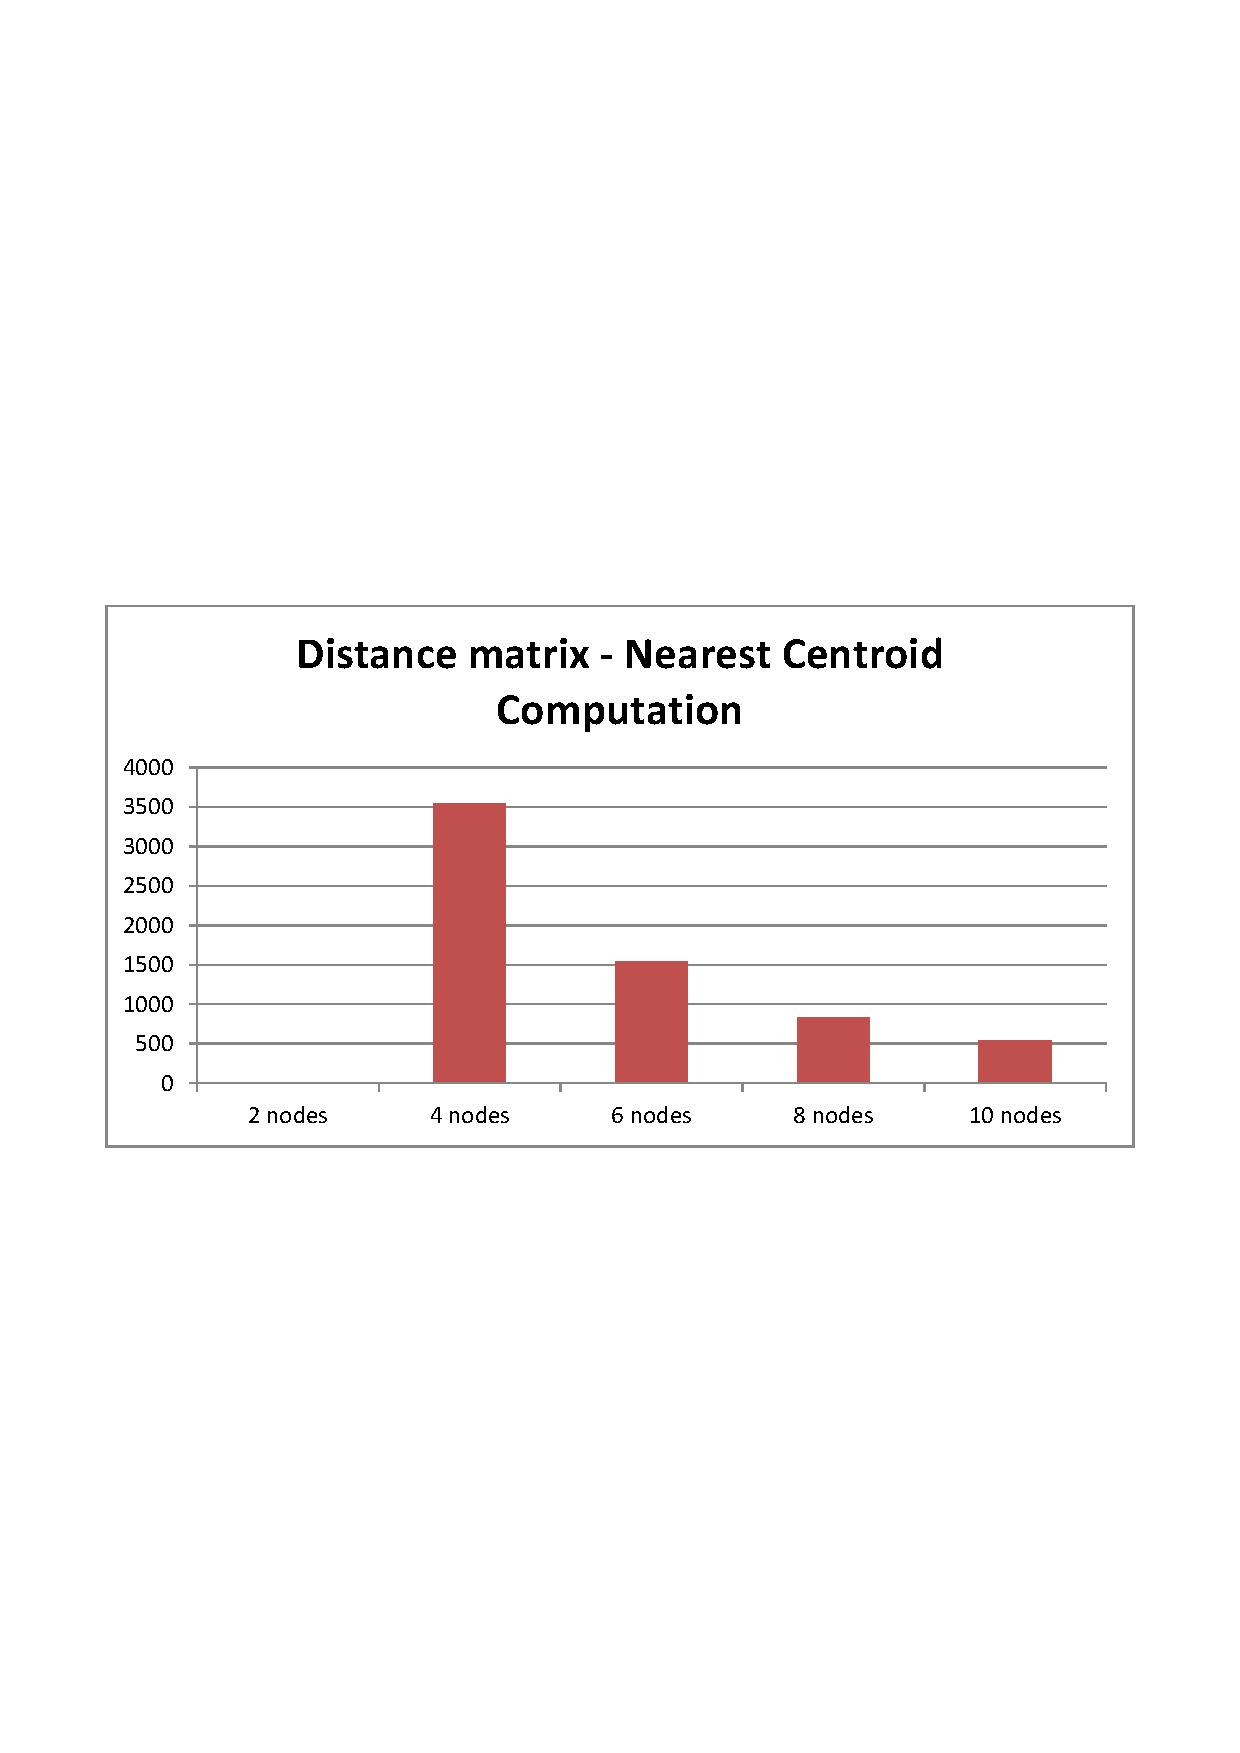
\includegraphics[trim = 10mm 90mm 10mm 90mm, clip, width=0.75\textwidth]{Figures/experiments/nearestcentroid_dist.pdf}
\caption{This figures shows the execution time when using the distance matrix method, when computing the nearest centroid.}
\label{fig:results_nearestcentroiddist}
\end{figure}

